\documentclass[10pt,a4paper]{article}

\usepackage[utf8]{inputenc}
\usepackage[english]{babel}
\usepackage[english]{isodate}
\usepackage[parfill]{parskip}
\usepackage{graphicx}
\usepackage{listings}
\usepackage{color}
\usepackage{authblk}

\usepackage{geometry}
 \geometry{
 a4paper,
 total={170mm,257mm},
 left=25mm,
 right=20mm,
 top=20mm,
 }

\usepackage{fancyhdr} % http://ctan.org/pkg/fancyhdr
\pagestyle{fancy} % Change page style to fancy
\usepackage{mdframed}
\usepackage[titletoc,title]{appendix}
\addto{\captionsenglish}{\renewcommand*{\appendixname}{Appendix}}

\definecolor{dkgreen}{rgb}{0,0.6,0}
\definecolor{gray}{rgb}{0.4,0.4,0.4}
\definecolor{mauve}{rgb}{0.58,0,0.82}
\definecolor{lightgray}{rgb}{0.97,0.97,0.97}

\mdfdefinestyle{bgbox}{backgroundcolor=lightgray,
  topline=false,bottomline=false,rightline=false,
  linecolor=lightgray,linewidth=7pt,leftmargin=-15pt}

% Code snippets
%\def\lstsetc{\lstset{language=C,
\lstset{frame=tb,
  language=C,
  aboveskip=3mm,
  belowskip=3mm,
  showstringspaces=false,
  columns=flexible,
  basicstyle={\small\ttfamily},
  numbers=left,
  numberstyle=\tiny\color{gray},
  keywordstyle=\color{blue},
  commentstyle=\color{dkgreen},
  stringstyle=\color{mauve},
  breaklines=true,
  breakatwhitespace=true
  tabsize=3
  morekeywords={main, size_t, malloc, free,
    hsize_t, hid_t, herr_t,
    H5VL_class_value_t,
    H5VL_attr_class_t,
    H5VL_dataset_class_t,
    H5VL_datatype_class_t,
    H5VL_file_class_t,
    H5VL_group_class_t,
    H5VL_link_class_t,
    H5VL_object_class_t,
    H5VL_async_class_t,
    H5VL_class_t
    }
}

\title{HDF5 Virtual Object Layer (VOL)\\
    Connector Author Guide}

\author{The HDF Group}


\begin{document}

\maketitle
\thispagestyle{empty}

\vfill
\begin{center}

\includegraphics[width=4cm]{THG_LOGO.pdf} % also works with logo.pdf
\end{center}
\vfill
\vfill

\newpage
\pagenumbering{Roman}
\tableofcontents
\newpage

\pagenumbering{arabic}

\renewcommand\appendixtocname{Appendix}


%%% Local Variables: 
%%% mode: latex
%%% TeX-master: t
%%% End: 

\section{Introduction}
The Virtual Object Layer (VOL) is an abstraction layer in the HDF5
library that intercepts all API calls that could potentially access
objects in an HDF5 container and forwards those calls to plugin
''object drivers''. The plugins could store the objects in variety of
ways. A plugin could, for example, have objects be distributed
remotely over different platforms, provide a raw mapping of the model
to the file system, or even store the data in other file formats (like
native netCDF or HDF4 format). The user still gets the same data model
where access is done to a single HDF5 “container”; however the plugin
object driver translates from what the user sees to how the data is
actually stored. Having this abstraction layer maintains the object
model of HDF5 and would allow HDF5 developers or users to write their
own plugins for accessing HDF5 data.

This user guide is for developers interested in developing a VOL
plugin for the HDF5 library. The document is meant to be used in
conjunction with the HDF5 reference manual. It is assumed that the
reader has good knowledge of the VOL architecture obtained by reading
the VOL architectural design document~\cite{vol:rfc}. The
document will cover the steps needed to create external and internal
VOL plugins. Both ways have a lot of common steps and rules that will
be covered first.

\newpage
\section{Creating a VOL Plugin}
\label{sec:vol}
Each VOL plugin should be of type {\tt H5VL\_class\_t} that is defined
as:

\begin{lstlisting}
/* Class information for each VOL driver */
typedef struct H5VL_class_t {
    H5VL_class_value_t value;
    const char *name;
    herr_t  (*initialize)(hid_t vipl_id);
    herr_t  (*terminate)(hid_t vtpl_id);
    size_t  fapl_size;
    void *  (*fapl_copy)(const void *info);
    herr_t  (*fapl_free)(void *info);

    /* Data Model */
    H5VL_attr_class_t          attr_cls;
    H5VL_dataset_class_t       dataset_cls;
    H5VL_datatype_class_t      datatype_cls;
    H5VL_file_class_t          file_cls;
    H5VL_group_class_t         group_cls;
    H5VL_link_class_t          link_cls;
    H5VL_object_class_t        object_cls;

    /* Services */
    H5VL_async_class_t         async_cls;
    herr_t (*optional)(void *obj, hid_t dxpl_id, void **req, va_list arguments);
} H5VL_class_t;
\end{lstlisting}

The {\tt value} field is a unique integer enum identifier that should be
greater than 128 for external plugins and smaller than 128 for
internal plugins. Setting it in the VOL structure is required.

The {\tt name} field is a string that uniquely identifies the VOL plugin
name. Setting it in the VOL structure is required. No two plugins with the same name can be registered with the library at the same time.

The {\tt initialize} field is a function pointer to a routine that a plugin implements to set up or intialize access to the plugin. Implementing this function by the plugin is not required, since some plugins do not require any set up to start accessing the plugin. In that case, the value of the function pointer should be set to NULL. Plugin specific variables that are required to be passed from users should be passed through the VOL initialize property list. Generic properties can be added to this property class for user-defined plugins that can not modify the HDF5 library to add internal properties. For more information consult the property list reference manual pages.

The {\tt terminate} field is a function pointer to a routine that a plugin implements to terminate or finalize access to the plugin. Implementing this function by the plugin is not required, since some plugins do not require any termination phase to the plugin. In that case, the value of the function pointer should be set to NULL. Plugin specific variables that are required to be passed from users should be passed through the VOL terminate property list. Generic properties can be added to this property class for user-defined plugins that can not modify the HDF5 library to add internal properties. For more information consult the property list reference manual pages.

The {\tt fapl\_size} field indicates the size required to store the
info data that the plugin needs. That info data is passed when the
plugin is selected for usage with the file access property list (fapl)
function. It might be that the plugin defined does not require any
information from the user, which means the size in this field will be
zero. More information about the info data and the fapl selection
routines follow later.

The {\tt fapl\_copy} field is a function pointer that is called when
the plugin is selected with the fapl function. It allows the plugin to
make a copy if the info data since the user might free it when closing
the fapl. It is required if there is info data needed by the plugin.

The {\tt fapl\_free} field is a function pointer that is called to
free the info data when the fapl close routine is called. It is
required if there is info data needed by the plugin.

The rest of the fields in the {\tt H5VL\_class\_t} struct are "subclasses'' that define all the VOL function callbacks that
are mapped to from the HDF5 API layer. Those subclasses are categorized into two categories, Data Model and Services. Data Model classes are those that provide functionality for accessing an HDF5 container and objects in that container as defined by the HDF5 data model.  Service classes are those that provide services for users that are not related to the data model specifically. Asynchronous operations, for example, are a service that most plugins can implement, so we add a class for it in the VOL structure. If a service becomes generic enough and common between many plugins, a class for it should be added in the VOL structure. However, many plugins can/will provide services that are not shared by other plugins. A good way to support these services is through an optional callback in the VOL structure which can be a hook from the API to the plugin that provides those services, passing any necessary arguments needed without the HDF5 library having to worry about supporting that service. A similar API operation to allow users to use that service will be added. This API call would be similar to an “ioctl” call where any kind of operation can be supported and passed down to the plugin that has enough knowledge from the user to interpret the type of the operation. All classes and their defined callbacks will be detailed in the following sub-sections.

\subsection{Mapping the API to the Callbacks}
\label{sec:map}

The callback interface defined for the VOL has to be general enough to
handle all the HDF5 API operations that would access the
file. Furthermore it has to capture future additions to the HDF5
library with little to no changes to the callback interface. Changing
the interface often whenever new features are added would be
discouraging to plugin developers since that would mean reworking
their VOL plugin structure. To remedy this issue, every callback will
contain two parameters:
\begin{itemize}
\item A data transfer property list (DXPL) which allows that API to
  put some properties on for the plugins to retrieve if they have to
  for particular operations, without having to add arguments to the
  VOL callback function.
\item A pointer to a request ({\tt void **req}) to handle asynchronous
  operations if the HDF5 library adds support for them in future
  releases (beyond the 1.8 series). That pointer is set by the VOL
  plugin to a request object it creates to manage progress on that
  asynchronous operation. If the {\tt req} is {\tt NULL}, that means
  that the API operation is blocking and so the plugin would not
  execute the operation asynchronously. If the plugin does not support
  asynchronous operations, it needs not to worry about this field and
  leaves it unset.
\end{itemize}

In order to keep the number of the VOL object classes and callbacks
concise and readable, it was decided to not have a one-to-one mapping
between API operation and callbacks. Furthermore, to keep the
callbacks themselves short and not cluttered with a lot of parameters,
some of the parameters are passed in as properties in property lists
included with the callback. The value of those properties can be
retrieved by calling the public routine (or its private version if
this is an internal plugin): 
\begin{lstlisting}
herr_t H5Pget(hid_t plist_id, const char *property_name, void *value);
\end{lstlisting}
The property names and value types will be detailed when describing
each callback in their respective sections.

The HDF5 library provides several routines to access an object in the
container. For example to open an attribute on a group object, the
user could use {\tt H5Aopen()} and pass the group identifier directly
where the attribute needs to be opened. Alternatively, the user could
use {\tt H5Aopen\_by\_name()} or {\tt H5Aopen\_by\_idx()} to open the
attribute, which provides a more flexible way of locating the
attribute, whether by a starting object location and a path or an
index type and traversal order. All those types of accesses usually
map to one VOL callback with a parameter that indicates the access
type. In the example of opening an attribute, the three API open
routine will map to the same VOL open callback but with a different
location parameter. The same applies to all types of routines that
have multiple types of accesses.  The location parameter is a
structure defined as follows:

\begin{lstlisting}
/* 
 * Structure to hold parameters for object locations.
 * either: BY_SELF, BY_NAME, BY_IDX, BY_ADDR, BY_REF 
 */

typedef struct H5VL_loc_params_t {
    H5I_type_t obj_type; /* The object type of the location object */
    H5VL_loc_type_t type; /* The location type */
    union { /* parameters of the location */
        struct H5VL_loc_by_name loc_by_name;
        struct H5VL_loc_by_idx  loc_by_idx;
        struct H5VL_loc_by_addr loc_by_addr;
        struct H5VL_loc_by_ref  loc_by_ref;
    }loc_data;
} H5VL_loc_params_t

/* 
 * Types for different ways that objects are located in an 
 * HDF5 container.
 */
typedef enum H5VL_loc_type_t {
    /* starting location is the target object*/
    H5VL_OBJECT_BY_SELF, 

    /* location defined by object and path in H5VL_loc_by_name */
    H5VL_OBJECT_BY_NAME, 

    /* location defined by object, path, and index in H5VL_loc_by_idx */
    H5VL_OBJECT_BY_IDX,

    /* location defined by physical address in H5VL_loc_by_addr */
    H5VL_OBJECT_BY_ADDR,

    /* NOT USED */
    H5VL_OBJECT_BY_REF
} H5VL_loc_type_t;

struct H5VL_loc_by_name {
    const char *name; /* The path relative to the starting location */
    hid_t plist_id; /* The link access property list */
};

struct H5VL_loc_by_idx {
    const char *name; /* The path relative to the starting location */
    H5_index_t idx_type; /* Type of index */
    H5_iter_order_t order; /* Index traversal order */
    hsize_t n; /* position in index */
    hid_t plist_id; /* The link access property list */
};

struct H5VL_loc_by_addr {
    haddr_t addr; /* physical address of location */
};

/* Not used for now */
struct H5VL_loc_by_ref {
    H5R_type_t ref_type;
    const void *_ref;
    hid_t plist_id;
};
\end{lstlisting}

Other API routines that would make a one-to-one mapping difficult are:
\begin{itemize} 
\item the {\tt Get} operations that retrieve something from an object; for example a property list or a datatype of a dataset, etc... 
\item API routines specific to each class of callbacks(attributes, files, etc...). Having a callback for each one would clutter the VOL callback structure and reduce user friendliness. 
\item API routines that make sense to only implement in the native HDF5 file format and would not be possible to implement in other plugins. Adding a callback for those routines would be confusing to plugin developers. 
\end{itemize}

To handle that large set of API routines, each class in the Data Model category has three generic callbacks, {\tt get}, {\tt specific}, and {\tt optional} to handle the three set of API operations outline above respectively. The callbacks will have a {\tt va\_list} argument to handle the different set of parameters that could be passed in.  The {\tt get} and {\tt specific} callbacks also have an {\tt op\_type} that contain an {\tt enum} of the type of operation that is requested to be performed. Using that type, the {\tt va\_list} argument can be parsed. The {\tt optional} callback is a free for all callback where anything from the API layer is passed in directly. This callback is used to support plugin specific operations in the API that other plugins should or would not know about. More information about types and the arguments for each type will be detailed in the corresponding class arguments.


\subsection{The File Function Callbacks}
The file API routines (H5F) allow HDF5 users to create and manage HDF5
containers. All the H5F API routines that modify the HDF5 container
map to one of the file callback routines in this class that the plugin
needs to implement:

\begin{lstlisting}
typedef struct H5VL_file_class_t {
    void *(*create)(const char *name, unsigned flags, hid_t fcpl_id, hid_t fapl_id, hid_t dxpl_id, void **req);
    void *(*open)(const char *name, unsigned flags, hid_t fapl_id, hid_t dxpl_id, void **req);
    herr_t (*get)(void *obj, H5VL_file_get_t get_type, hid_t dxpl_id, void **req, va_list arguments);
    herr_t (*specific)(void *obj, H5VL_file_specific_t specific_type, hid_t dxpl_id, void **req, va_list arguments);
    herr_t (*optional)(void *obj, hid_t dxpl_id, void **req, va_list arguments);
    herr_t (*close) (void *file, hid_t dxpl_id, void **req);
} H5VL_file_class_t;
\end{lstlisting}

The {\tt create} callback in the file class should create a container
and returns a pointer to the file structure created by the plugin containing information to
access the container in future calls.

\textbf{Signature:}
\begin{lstlisting}
    void *(*create)(const char *name, unsigned flags, hid_t fcpl_id, hid_t fapl_id, hid_t dxpl_id, void **req);
\end{lstlisting}

\textbf{Arguments:}\\
\begin{tabular}{l p{10cm}}
  {\tt name} & (IN): The name of the container to be created.\\
  {\tt flags} & (IN): The creation flags of the container.\\
  {\tt fcpl\_id} & (IN): The file creation property list.\\
  {\tt fapl\_id} & (IN): The file access property list.\\
  {\tt dxpl\_id} & (IN): The data transfer property list.\\
  {\tt req} & (IN/OUT): A pointer to the asynchronous request of the
  operation created by the plugin.\\
\end{tabular}

The {\tt open} callback in the file class should open a container and
returns a pointer to the file structure created by the plugin containing information to
access the container in future calls.

\textbf{Signature:}
\begin{lstlisting}
    void *(*open)(const char *name, unsigned flags, hid_t fapl_id, hid_t dxpl_id, void **req);
\end{lstlisting}

\textbf{Arguments:}\\
\begin{tabular}{l p{10cm}}
  {\tt name} & (IN): The name of the container to open.\\
  {\tt flags} & (IN): The open flags of the container.\\
  {\tt fapl\_id} & (IN): The file access property list.\\
  {\tt dxpl\_id} & (IN): The data transfer property list.\\
  {\tt req} & (IN/OUT): A pointer to the asynchronous request of the
  operation created by the plugin.\\
\end{tabular}

The {\tt get} callback in the file class should retrieve
information about the container as specified in the {\tt get\_type}
parameter. It returns an {\tt herr\_t} indicating success or failure.

\textbf{Signature:}
\begin{lstlisting}
    herr_t (*get)(void *obj, H5VL_file_get_t get_type, hid_t dxpl_id, 
        void **req, va_list arguments);
\end{lstlisting}

The {\tt get\_type} argument is an {\tt enum}:
\begin{lstlisting}
/* types for all file get API routines */
typedef enum H5VL_file_get_t {
    H5VL_FILE_GET_FAPL,      /* file access property list   */
    H5VL_FILE_GET_FCPL,      /* file creation property list */
    H5VL_FILE_GET_INTENT,    /* file intent                 */
    H5VL_FILE_GET_NAME,      /* file name                   */
    H5VL_FILE_GET_OBJ_COUNT, /* object count in file        */
    H5VL_FILE_GET_OBJ_IDS,   /* object ids in file          */
    H5VL_OBJECT_GET_FILE     /* retrieve or resurrect file of object */
} H5VL_file_get_t;
\end{lstlisting}

\textbf{Arguments:}\\
\begin{tabular}{l p{10cm}}
  {\tt obj} & (IN): The container or object where information needs to be
  retrieved from.\\
  {\tt get\_type} & (IN): The type of the information to retrieve.\\
  {\tt dxpl\_id} & (IN): The data transfer property list.\\
  {\tt req} & (IN/OUT): A pointer to the asynchronous request of the
  operation created by the plugin.\\
  {\tt arguments} & (IN/OUT): argument list containing parameters and
  output pointers for the get operation. \\
\end{tabular}

The {\tt arguments} argument contains a variable list of arguments
depending on the {\tt get\_type} parameter. The following list shows
the argument list, in-order, for each type:

\begin{itemize}
\item {\tt H5VL\_FILE\_GET\_FCPL}, to retrieve the file creation
  property list:
  \begin{enumerate}
  \item {\tt hid\_t *ret\_id} (OUT): buffer for the identifier of the
    file creation property list.
  \end{enumerate}

\item {\tt H5VL\_FILE\_GET\_FAPL}, to retrieve the file access
  property list:
  \begin{enumerate}
  \item {\tt hid\_t *ret\_id} (OUT): buffer for the identifier of the
    file access property list.
  \end{enumerate}

\item {\tt H5VL\_FILE\_GET\_OBJ\_COUNT:}, to retrieve the object count
  in the container:
  \begin{enumerate}
  \item {\tt unsigned types} (IN): type of objects to look for.
  \item {\tt ssize\_t *ret} (OUT): buffer for the object count.
  \end{enumerate}

\item {\tt H5VL\_FILE\_GET\_OBJ\_IDS:}, to retrieve object identifiers
  in the container:
  \begin{enumerate}
  \item {\tt unsigned types} (IN): type of objects to look for.
  \item {\tt size\_t max\_objs} (IN): maximum number of objects to
    open.
  \item {\tt hid\_t *oid\_list} (OUT): buffer for the object identifiers.
  \item {\tt ssize\_t *ret} (OUT): buffer for the object count.
  \end{enumerate}

\item {\tt H5VL\_FILE\_GET\_INTENT}, get access intent of the
  container:
  \begin{enumerate}
  \item {\tt unsigned *ret} (OUT): buffer for the intent value.
  \end{enumerate}

\item {\tt H5VL\_FILE\_GET\_NAME}, get container name an object
  belongs to:
  \begin{enumerate}
  \item {\tt H5I\_type\_t type} (IN): the object type in {\tt obj}.
  \item {\tt size\_t size} (IN): size of the buffer for the file name.
  \item {\tt char *name} (OUT): buffer for the file name.
  \item {\tt ssize\_t *ret} (OUT): buffer for the entire size of the
    file name.
  \end{enumerate}

\item {\tt H5VL\_OBJECT\_GET\_FILE}, get the container that the object
  belongs to:
  \begin{enumerate}
  \item {\tt H5I\_type\_t type} (IN): the object type in {\tt obj}.
  \item {\tt void **ret} (OUT): pointer to the file structure returned
    by the plugin.
  \end{enumerate}
\end{itemize}

The {\tt specific} callback in the file class implements specific operations on HDF5 files as specified in the {\tt
  specific\_type} parameter. It returns an {\tt herr\_t} indicating success or failure.

\textbf{Signature:}
\begin{lstlisting}
    herr_t (*specific)(void *obj, H5VL_file_specific_t specific_type, hid_t dxpl_id, void **req, va_list arguments);
\end{lstlisting}

The {\tt specific\_type} argument is an {\tt enum}:
\begin{lstlisting}
/* types for file SPECIFIC callback */
typedef enum H5VL_file_specific_t {
    H5VL_FILE_FLUSH,                  /* Flush file */
    H5VL_FILE_IS_ACCESSIBLE,          /* Check if a file is accessible */
    H5VL_FILE_MOUNT,                  /* Mount a file */
    H5VL_FILE_UNMOUNT                 /* Un-Mount a file */
} H5VL_file_specific_t;
\end{lstlisting}

\textbf{Arguments:}\\
\begin{tabular}{l p{10cm}}
  {\tt obj} & (IN): The container or object where the operation needs
  to happen.\\
  {\tt specific\_type} & (IN): The type of the operation.\\
  {\tt dxpl\_id} & (IN): The data transfer property list.\\
  {\tt req} & (IN/OUT): A pointer to the asynchronous request of the
  operation created by the plugin.\\
  {\tt arguments} & (IN/OUT): argument list containing parameters and
  output pointers for the get operation. \\
\end{tabular}

The {\tt arguments} argument contains a variable list of arguments
depending on the {\tt specific\_type} parameter. The following list shows
the argument list, in-order, for each type:

\begin{itemize}
\item {\tt H5VL\_FILE\_FLUSH}, flushes all buffers associated with the container to disk:
  \begin{enumerate}
  \item {\tt H5I\_type\_t obj\_type} (IN): The object type of {\tt obj} on which the flush operation was called.
  \item {\tt H5F\_scope\_t scope} (IN): The scope of the flushing action.
  \end{enumerate}
  
\item {\tt H5VL\_FILE\_IS\_ACCESSIBLE}, checks if a container is
  accessible using a specific file access property list:
  \begin{enumerate}
  \item {\tt hid\_t *fapl\_id} (IN): file access property list.
  \item {\tt char *name} (IN): name of the container to check.
  \item {\tt htri\_t *result} (OUT): buffer for the result; 0 if no, 1
    if yes.
  \end{enumerate}
  
\item {\tt H5VL\_FILE\_MOUNT}, Mounts a file on the location object:
  \begin{enumerate}
  \item {\tt H5I\_type\_t type} (IN): the object type in {\tt obj}.
  \item {\tt char *name} (IN): name of the group onto which the file
    specified by {\tt file} is to be mounted.
  \item {\tt void *file} (IN): child file to be mounted.
  \item {\tt hid\_t *fmpl\_id} (IN): file mount property list.
  \end{enumerate}

\item {\tt H5VL\_FILE\_UNMOUNT}, un-mounts a file from the location object:
  \begin{enumerate}
  \item {\tt H5I\_type\_t type} (IN): the object type in {\tt obj}.
  \item {\tt char *name} (IN): name of the mount point.
  \end{enumerate}
\end{itemize}

The {\tt optional} callback in the file class implements plugin specific operations on an HDF5 container. It returns an {\tt
  herr\_t} indicating success or failure. 

\textbf{Signature:}
\begin{lstlisting}
    herr_t (*optional)(void *obj, hid_t dxpl_id, void **req, va_list arguments);
\end{lstlisting}

\textbf{Arguments:}\\
\begin{tabular}{l p{10cm}}
  {\tt obj} & (IN): The container or object where the operation needs to happen.\\
  {\tt dxpl\_id} & (IN): The data transfer property list.\\
  {\tt req} & (IN/OUT): A pointer to the asynchronous request of the operation created by the plugin.\\
  {\tt arguments} & (IN/OUT): argument list containing parameters and output pointers for the get operation. \\
\end{tabular}

Each plugin should be able to parse the {\tt va\_list arguments} if it has plugin specific operations to implement and determine the type of the operation and the parameters through a predefined schema. For example, in the native plugin, the first argument in the {\tt va\_list} is the optional argument type enum defined as follows:

\begin{lstlisting}
/* types for all file optional operations */
typedef enum H5VL_file_optional_t {
    H5VL_FILE_CLEAR_ELINK_CACHE,  /* Clear external link cache         */
    H5VL_FILE_GET_FILE_IMAGE,     /* file image                        */
    H5VL_FILE_GET_FREE_SECTIONS,  /* file free selections              */
    H5VL_FILE_GET_FREE_SPACE,     /* file freespace                    */
    H5VL_FILE_GET_INFO,           /* file info                         */
    H5VL_FILE_GET_MDC_CONF,       /* file metadata cache configuration */
    H5VL_FILE_GET_MDC_HR,         /* file metadata cache hit rate      */
    H5VL_FILE_GET_MDC_SIZE,       /* file metadata cache size          */
    H5VL_FILE_GET_SIZE,           /* file size                         */
    H5VL_FILE_GET_VFD_HANDLE,     /* file VFD handle                   */
    H5VL_FILE_REOPEN,             /* reopen the file                   */
    H5VL_FILE_RESET_MDC_HIT_RATE, /* get metadata cache hit rate       */
    H5VL_FILE_SET_MDC_CONFIG      /* set metadata cache configuration  */
} H5VL_file_optional_t;
\end{lstlisting}

The remaining arguments are parsed depending on the optional operation type.


%\begin{itemize}
%
%\item {\tt H5VL\_FILE\_GET\_SIZE}, retrieve the size of the container
%  in {\tt obj}:
%  \begin{enumerate}
%  \item {\tt hsize\_t *ret} (OUT): file size.
%  \end{enumerate}
%
%\item {\tt H5VL\_FILE\_GET\_FILE\_IMAGE}, retrieve file image from the
%  container in {\tt obj}:
%  \begin{enumerate}
%  \item {\tt void *buf\_ptr} (OUT): buffer to return the file image.
%  \item {\tt ssize\_t *ret} (OUT): buffer for the total size needed for
%    the file image.
%  \item {\tt size\_t buf\_len} (IN): size of the buffer passed in.
%  \end{enumerate}
%
%\item {\tt H5VL\_FILE\_GET\_FREE\_SPACE}, retrieve amount of free
%  space in the container in {\tt obj}:
%  \begin{enumerate}
%  \item {\tt hssize\_t *ret} (OUT): buffer for the free space.
%  \end{enumerate}
%
%\item {\tt H5VL\_FILE\_GET\_FREE\_SECTIONS}, retrieve free sections from the
%  container in {\tt obj}:
%  \begin{enumerate}
%  \item {\tt H5F\_sect\_info\_t *sinfo} (OUT): pointer to the section
%    info structure to fill.
%  \item {\tt ssize\_t *ret} (OUT): buffer for the total number of free
%    sections.
%  \item {\tt H5F\_mem\_t type} (IN): type of the memory space to check
%    for.
%  \item {\tt size\_t nsects} (IN): number of section allocate in {\tt sinfo}.
%  \end{enumerate}
%
%\item {\tt H5VL\_FILE\_GET\_INFO}, retrieve file info from the
%  object in {\tt obj}:
%  \begin{enumerate}
%  \item {\tt H5I\_type\_t type} (IN): the object type in {\tt obj}.
%  \item {\tt H5F\_info2\_t *finfo} (OUT): pointer to info structure to fill.
%  \end{enumerate}
%
%\item {\tt H5VL\_FILE\_GET\_MDC\_CONF}, retrieve the meta data cache
%  configuration from the container in {\tt obj}:
%  \begin{enumerate}
%  \item {\tt H5I\_type\_t type} (IN): the object type in {\tt obj}.
%  \item {\tt H5AC\_cache\_config\_t *conf} (OUT): pointer to
%    configuration structure to fill.
%  \end{enumerate}
%
%\item {\tt H5VL\_FILE\_GET\_MDC\_HR}, retrieve the meta data cache
%  hit rate from the container in {\tt obj}:
%  \begin{enumerate}
%  \item {\tt double *ret} (OUT): buffer for the hit rate.
%  \end{enumerate}
%
%\item {\tt H5VL\_FILE\_GET\_MDC\_SIZE}, retrieve the meta data cache
%  size information from the container in {\tt obj}:
%  \begin{enumerate}
%  \item {\tt size\_t max\_size\_ptr} (OUT): buffer for maximum size.
%  \item {\tt size\_t min\_clean\_size\_ptr} (OUT): buffer for minimum
%    clean size.
%  \item {\tt size\_t cur\_size\_ptr} (OUT): buffer for current size.
%  \item {\tt int cur\_num\_entries\_ptr} (OUT): buffer for number of
%    current cache entries.
%  \end{enumerate}
%
%\item {\tt H5VL\_FILE\_GET\_VFD\_HANDLE}, retrieve the virtual file
%  driver handle from the container in {\tt obj}:
%  \begin{enumerate}
%  \item {\tt void **handle} (OUT): pointer to a buffer the plugin sets
%    to the VFD handle.
%  \item {\tt hid\_t fapl} (IN): File access property list.
%  \end{enumerate}
%
%\item {\tt H5VL\_FILE\_CLEAR\_ELINK\_CACHE}, clears the external link
%  file cache. Takes no extra arguments.
%
%\item {\tt H5VL\_FILE\_REOPEN}, reopen the container in {\tt obj}:
%  \begin{enumerate}
%  \item {\tt void **ret} (OUT): pointer to be set to the opened file
%    structure.
%  \end{enumerate}
%
%\item {\tt H5VL\_FILE\_RESET\_MDC\_HIT\_RATE}, resets the hit rate
%  statistics for the metadata cache on the container in {\tt
%    obj}. Takes no extra arguments.
%
%\item {\tt H5VL\_FILE\_SET\_MDC\_CONFIG}, sets the meta data cache
%  configuration for the container in {\tt obj}:
%  \begin{enumerate}
%  \item {\tt H5AC\_cache\_config\_t *conf} (IN): pointer to
%    configuration structure to use.
%  \end{enumerate}
%
%\end{itemize}

The {\tt close} callback in the file class should terminate access to
the file object and free all resources it was consuming, and returns
an {\tt herr\_t} indicating success or failure.

\textbf{Signature:}
\begin{lstlisting}
    herr_t (*close)(void *file, hid_t dxpl_id, void **req);
\end{lstlisting}

\textbf{Arguments:}\\
\begin{tabular}{l p{10cm}}
  {\tt file} & (IN): Pointer to the file.\\
  {\tt dxpl\_id} & (IN): The data transfer property list.\\
  {\tt req} & (IN/OUT): A pointer to the asynchronous request of the
  operation created by the plugin.\\
\end{tabular}

\subsection{The Group Function Callbacks}
The group API routines (H5G) allow HDF5 users to create and manage
HDF5 groups. All the H5G API routines that modify the HDF5 container
map to one of the group callback routines in this class that the
plugin needs to implement:

\begin{lstlisting}
typedef struct H5VL_group_class_t {
    void *(*create)(void *obj, H5VL_loc_params_t loc_params, const char *name, hid_t gcpl_id, hid_t gapl_id, hid_t dxpl_id, void **req);
    void *(*open)(void *obj, H5VL_loc_params_t loc_params, const char *name, hid_t gapl_id, hid_t dxpl_id, void **req);
    herr_t (*get)(void *obj, H5VL_group_get_t get_type, hid_t dxpl_id, void **req, va_list arguments);
    herr_t (*specific)(void *obj, H5VL_group_specific_t specific_type, hid_t dxpl_id, void **req, va_list arguments);
    herr_t (*optional)(void *obj, hid_t dxpl_id, void **req, va_list arguments);
    herr_t (*close) (void *grp, hid_t dxpl_id, void **req);
} H5VL_group_class_t;
\end{lstlisting}

The {\tt create} callback in the group class should create a group
object in the container of the location object and returns a pointer
to the group structure containing information to access the group in
future calls.

\textbf{Signature:}
\begin{lstlisting}
    void *(*create)(void *obj, H5VL_loc_params_t loc_params, const char *name, hid_t gcpl_id, hid_t gapl_id, hid_t dxpl_id, void **req);
\end{lstlisting}

\textbf{Arguments:}\\
\begin{tabular}{l p{10cm}}
  {\tt obj} & (IN): Pointer to an object where the group needs
  to be created or where the look-up of the target object needs to
  start.\\
  {\tt loc\_params} & (IN): The location parameters as explained in
  section~\ref{sec:map}. The type can be only {\tt
    H5VL\_OBJECT\_BY\_SELF} in this callback. \\
  {\tt name} & (IN): The name of the group to be created.\\
  {\tt dcpl\_id} & (IN): The group creation property list. It contains
  all the group creation properties in addition to the link creation
  property list of the create operation (an {\tt hid\_t}) that can be
  retrieved with the property {\tt H5VL\_GRP\_LCPL\_ID}.\\
  {\tt gapl\_id} & (IN): The group access property list.\\
  {\tt dxpl\_id} & (IN): The data transfer property list.\\
  {\tt req} & (IN/OUT): A pointer to the asynchronous request of the
  operation created by the plugin.\\
\end{tabular}

The {\tt open} callback in the group class should open a group object
in the container of the location object and returns a pointer to the
group structure containing information to access the group in future
calls.

\textbf{Signature:}
\begin{lstlisting}
    void *(*open)(void *obj, H5VL_loc_params_t loc_params, 
        const char*name, hid_t gapl_id, hid_t dxpl_id, void **req);
\end{lstlisting}

\textbf{Arguments:}\\
\begin{tabular}{l p{10cm}}
  {\tt obj} & (IN): Pointer to an object where the group needs to be
  opened or where the look-up of the target object needs to start.\\
  {\tt loc\_params} & (IN): The location parameters as explained in
  section~\ref{sec:map}. The type can be only {\tt
    H5VL\_OBJECT\_BY\_SELF} in this callback. \\
  {\tt name} & (IN): The name of the group to be opened.\\
  {\tt dapl\_id} & (IN): The group access property list.\\
  {\tt dxpl\_id} & (IN): The data transfer property list.\\
  {\tt req} & (IN/OUT): A pointer to the asynchronous request of the
  operation created by the plugin.\\
\end{tabular}

The {\tt get} callback in the group class should retrieve information
about the group as specified in the {\tt get\_type} parameter. It
returns an {\tt herr\_t} indicating success or failure.

\textbf{Signature:}
\begin{lstlisting}
    herr_t (*get)(void *obj, H5VL_group_get_t get_type, hid_t dxpl_id, void **req, va_list arguments);
\end{lstlisting}

The {\tt get\_type} argument is an {\tt enum}:
\begin{lstlisting}
/* types for all group get API routines */
typedef enum H5VL_group_get_t {
    H5VL_GROUP_GET_GCPL,      /*group creation property list */
    H5VL_GROUP_GET_INFO       /*group info                   */
} H5VL_group_get_t;
\end{lstlisting}

\textbf{Arguments:}\\
\begin{tabular}{l p{10cm}}
  {\tt obj} & (IN): The group object where information needs to be
  retrieved from.\\
  {\tt get\_type} & (IN): The type of the information to retrieve.\\
  {\tt dxpl\_id} & (IN): The data transfer property list.\\
  {\tt req} & (IN/OUT): A pointer to the asynchronous request of the
  operation created by the plugin.\\
  {\tt arguments} & (IN/OUT): argument list containing parameters and
  output pointers for the get operation. \\
\end{tabular}

The {\tt arguments} argument contains a variable list of arguments
depending on the {\tt get\_type} parameter. The following list shows
the argument list, in-order, for each type:

\begin{itemize}
\item {\tt H5VL\_GROUP\_GET\_GCPL}, to retrieve the group creation
  property list of the group specified in {\tt obj}:
  \begin{enumerate}
  \item {\tt hid\_t *ret\_id} (OUT): buffer for the identifier of the
    group creation property list.
  \end{enumerate}

\item {\tt H5VL\_GROUP\_GET\_INFO}, to retrieve the attribute info:
  \begin{enumerate}
  \item {\tt H5VL\_loc\_params\_t loc\_params} (IN): The location parameters
    explained in section~\ref{sec:map}. 
  \item {\tt H5G\_info\_t *ginfo} (OUT): info structure to fill the
    group info in.
  \end{enumerate}
\end{itemize}

The {\tt specific} callback in the group class currently does not require any functionality to be implemented and should be left as {\tt NULL}.

The {\tt optional} callback in the group class implements plugin specific operations on an HDF5 group. It returns an {\tt
  herr\_t} indicating success or failure. 

\textbf{Signature:}
\begin{lstlisting}
    herr_t (*optional)(void *obj, hid_t dxpl_id, void **req, va_list arguments);
\end{lstlisting}

\textbf{Arguments:}\\
\begin{tabular}{l p{10cm}}
  {\tt obj} & (IN): The container or object where the operation needs to happen.\\
  {\tt dxpl\_id} & (IN): The data transfer property list.\\
  {\tt req} & (IN/OUT): A pointer to the asynchronous request of the operation created by the plugin.\\
  {\tt arguments} & (IN/OUT): argument list containing parameters and output pointers for the get operation. \\
\end{tabular}

Each plugin should be able to parse the {\tt va\_list arguments} if it has plugin specific operations to implement and determine the type of the operation and the parameters through a predefined schema. 

The {\tt close} callback in the group class should terminate access to
the group object and free all resources it was consuming, and returns
an {\tt herr\_t} indicating success or failure.

\textbf{Signature:}
\begin{lstlisting}
    herr_t (*close)(void *group, hid_t dxpl_id, void **req);
\end{lstlisting}

\textbf{Arguments:}\\
\begin{tabular}{l p{10cm}}
  {\tt group} & (IN): Pointer to the group object.\\
  {\tt dxpl\_id} & (IN): The data transfer property list.\\
  {\tt req} & (IN/OUT): A pointer to the asynchronous request of the
  operation created by the plugin.\\
\end{tabular}

\subsection{The Dataset Function Callbacks}
The dataset API routines (H5D) allow HDF5 users to create and manage
HDF5 datasets. All the H5D API routines that modify the HDF5 container
map to one of the dataset callback routines in this class that the
plugin needs to implement:

\begin{lstlisting}
typedef struct H5VL_dataset_class_t {
    void *(*create)(void *obj, H5VL_loc_params_t loc_params, const char *name, hid_t dcpl_id, hid_t dapl_id, hid_t dxpl_id, void **req);
    void *(*open)(void *obj, H5VL_loc_params_t loc_params, const char *name, hid_t dapl_id, hid_t dxpl_id, void **req);
    herr_t (*read)(void *dset, hid_t mem_type_id, hid_t mem_space_id, hid_t file_space_id, hid_t xfer_plist_id, void * buf, void **req);
    herr_t (*write)(void *dset, hid_t mem_type_id, hid_t mem_space_id, hid_t file_space_id, hid_t xfer_plist_id, const void * buf, void **req);
    herr_t (*get)(void *obj, H5VL_dataset_get_t get_type, hid_t dxpl_id, void **req, va_list arguments);
    herr_t (*specific)(void *obj, H5VL_dataset_specific_t specific_type, hid_t dxpl_id, void **req, va_list arguments);
    herr_t (*optional)(void *obj, hid_t dxpl_id, void **req, va_list arguments);
    herr_t (*close) (void *dset, hid_t dxpl_id, void **req);
} H5VL_dataset_class_t;
\end{lstlisting}

The {\tt create} callback in the dataset class should create a dataset
object in the container of the location object and returns a pointer
to the dataset structure containing information to access the dataset
in future calls.

\textbf{Signature:}
\begin{lstlisting}
    void *(*create)(void *obj, H5VL_loc_params_t loc_params, const char *name, hid_t dcpl_id, hid_t dapl_id, hid_t dxpl_id, void **req);
\end{lstlisting}

\textbf{Arguments:}\\
\begin{tabular}{l p{10cm}}
  {\tt obj} & (IN): Pointer to an object where the dataset needs
  to be created or where the look-up of the target object needs to
  start.\\
  {\tt loc\_params} & (IN): The location parameters as explained in
  section~\ref{sec:map}. The type can be only {\tt
    H5VL\_OBJECT\_BY\_SELF} in this callback. \\
  {\tt name} & (IN): The name of the dataset to be created.\\
  {\tt dcpl\_id} & (IN): The dataset creation property list. It contains
  all the dataset creation properties in addition to the dataset
  datatype (an {\tt hid\_t}), dataspace (an {\tt hid\_t}), and the
  link creation property list of the create operation (an {\tt
    hid\_t}) that can be retrieved with the properties, {\tt
    H5VL\_DSET\_TYPE\_ID}, {\tt H5VL\_DSET\_SPACE\_ID},  and {\tt
    H5VL\_DSET\_LCPL\_ID} respectively.\\
  {\tt dapl\_id} & (IN): The dataset access property list.\\
  {\tt dxpl\_id} & (IN): The data transfer property list.\\
  {\tt req} & (IN/OUT): A pointer to the asynchronous request of the
  operation created by the plugin.\\
\end{tabular}

The {\tt open} callback in the dataset class should open a dataset
object in the container of the location object and returns a pointer
to the dataset structure containing information to access the dataset
in future calls.

\textbf{Signature:}
\begin{lstlisting}
    void *(*open)(void *obj, H5VL_loc_params_t loc_params, const char *name, hid_t dapl_id, hid_t dxpl_id, void **req);
\end{lstlisting}

\textbf{Arguments:}\\
\begin{tabular}{l p{10cm}}
  {\tt obj} & (IN): Pointer to an object where the dataset needs to be
  opened or where the look-up of the target object needs to start.\\
  {\tt loc\_params} & (IN): The location parameters as explained in
  section~\ref{sec:map}. The type can be only {\tt
    H5VL\_OBJECT\_BY\_SELF} in this callback. \\
  {\tt name} & (IN): The name of the dataset to be opened.\\
  {\tt dapl\_id} & (IN): The dataset access property list.\\
  {\tt dxpl\_id} & (IN): The data transfer property list.\\
  {\tt req} & (IN/OUT): A pointer to the asynchronous request of the
  operation created by the plugin.\\
\end{tabular}

The {\tt read} callback in the dataset class should read data from
the dataset object and returns an {\tt herr\_t} indicating success or
failure.

\textbf{Signature:}
\begin{lstlisting}
    herr_t (*read)(void *dset, hid_t mem_type_id, hid_t mem_space_id, 
        hid_t file_space_id, hid_t dxpl_id, void *buf, void **req);
\end{lstlisting}

\textbf{Arguments:}\\
\begin{tabular}{l p{10cm}}
  {\tt dset} & (IN): Pointer to the dataset object.\\
  {\tt mem\_type\_id} & (IN): The memory datatype of the data.\\
  {\tt mem\_space\_id} & (IN): The memory dataspace selection.\\
  {\tt file\_space\_id} & (IN): The file dataspace selection.\\
  {\tt dxpl\_id} & (IN): The data transfer property list.\\
  {\tt buf} & (OUT): Data buffer to be read into.\\
  {\tt req} & (IN/OUT): A pointer to the asynchronous request of the
  operation created by the plugin.\\
\end{tabular}

The {\tt write} callback in the dataset class should write data to
the dataset object and returns an {\tt herr\_t} indicating success or
failure.

\textbf{Signature:}
\begin{lstlisting}
    herr_t (*write)(void *dset, hid_t mem_type_id, hid_t mem_space_id, 
        hid_t file_space_id, hid_t dxpl_id, const void * buf, void **req);
\end{lstlisting}

\textbf{Arguments:}\\
\begin{tabular}{l p{10cm}}
  {\tt dset} & (IN): Pointer to the dataset object.\\
  {\tt mem\_type\_id} & (IN): The memory datatype of the data.\\
  {\tt mem\_space\_id} & (IN): The memory dataspace selection.\\
  {\tt file\_space\_id} & (IN): The file dataspace selection.\\
  {\tt dxpl\_id} & (IN): The data transfer property list.\\
  {\tt buf} & (IN): Data buffer to be written from.\\
  {\tt req} & (IN/OUT): A pointer to the asynchronous request of the
  operation created by the plugin.\\
\end{tabular}

The {\tt get} callback in the dataset class should retrieve
information about the dataset as specified in the {\tt get\_type}
parameter.It returns an {\tt herr\_t} indicating success or failure.

\textbf{Signature:}
\begin{lstlisting}
    herr_t (*get)(void *dset, H5VL_dataset_get_t get_type, 
        hid_t dxpl_id, void **req, va_list arguments);
\end{lstlisting}

The {\tt get\_type} argument is an {\tt enum}:
\begin{lstlisting}
/* types for dataset GET callback */
typedef enum H5VL_dataset_get_t {
    H5VL_DATASET_GET_DAPL,                  /* access property list */
    H5VL_DATASET_GET_DCPL,                  /* creation property list */
    H5VL_DATASET_GET_OFFSET,                /* offset */
    H5VL_DATASET_GET_SPACE,                 /* dataspace */
    H5VL_DATASET_GET_SPACE_STATUS,          /* space  status */
    H5VL_DATASET_GET_STORAGE_SIZE,          /* storage size */
    H5VL_DATASET_GET_TYPE                   /* datatype */
} H5VL_dataset_get_t;
\end{lstlisting}

\textbf{Arguments:}\\
\begin{tabular}{l p{10cm}}
  {\tt dset} & (IN): The dataset object where information needs to be
  retrieved from.\\
  {\tt get\_type} & (IN): The type of the information to retrieve.\\
  {\tt dxpl\_id} & (IN): The data transfer property list.\\
  {\tt req} & (IN/OUT): A pointer to the asynchronous request of the
  operation created by the plugin.\\
  {\tt arguments} & (IN/OUT): argument list containing parameters and
  output pointers for the get operation. \\
\end{tabular}

The {\tt arguments} argument contains a variable list of arguments
depending on the {\tt get\_type} parameter. The following list shows
the argument list, in-order, for each type:

\begin{itemize}
\item {\tt H5VL\_DATASET\_GET\_DAPL}, to retrieve the dataset access
  property list of the dataset specified in {\tt obj}:
  \begin{enumerate}
  \item {\tt hid\_t *ret\_id} (OUT): buffer for the identifier of the
    dataset access property list.
  \end{enumerate}

\item {\tt H5VL\_DATASET\_GET\_DCPL}, to retrieve the dataset creation
  property list of the dataset specified in {\tt obj}:
  \begin{enumerate}
  \item {\tt hid\_t *ret\_id} (OUT): buffer for the identifier of the
    dataset creation property list.
  \end{enumerate}

\item {\tt H5VL\_DATASET\_GET\_OFFSET}, to retrieve the offset of the
  dataset specified in {\tt obj} in the container:
  \begin{enumerate}
  \item {\tt haddr\_t *ret} (OUT): buffer for the offset of the
    dataset in the container.
  \end{enumerate}

\item {\tt H5VL\_DATASET\_GET\_SPACE}, to retrieve the dataspace of the
  dataset specified in {\tt obj}:
  \begin{enumerate}
  \item {\tt hid\_t *ret\_id} (OUT): buffer for the identifier of the
    dataset dataspace.
  \end{enumerate}

\item {\tt H5VL\_DATASET\_GET\_SPACE\_STATUS}, to retrieve the
  information whether space has been allocated for the dataset:
  \begin{enumerate}
  \item {\tt H5D\_space\_status\_t *allocation} (OUT): buffer for the
    space status.
  \end{enumerate}

\item {\tt H5VL\_DATASET\_GET\_STORAGE\_SIZE}, to retrieve the storage
  size of the dataset specified in {\tt obj}:
  \begin{enumerate}
  \item {\tt hsize\_t *ret} (OUT): buffer for the storage size of
    the dataset in the container.
  \end{enumerate}

\item {\tt H5VL\_DATASET\_GET\_TYPE}, to retrieve the datatype of the
  dataset specified in {\tt obj}:
  \begin{enumerate}
  \item {\tt hid\_t *ret\_id} (OUT): buffer for the identifier of the
    dataset datatype.
  \end{enumerate}
\end{itemize}

The {\tt specific} callback in the dataset class implements specific operations on HDF5 datasets as specified in the {\tt
  specific\_type} parameter. It returns an {\tt herr\_t} indicating success or failure.

\textbf{Signature:}
\begin{lstlisting}
    herr_t (*specific)(void *obj, H5VL_file_specific_t specific_type, hid_t dxpl_id, void **req, va_list arguments);
\end{lstlisting}

The {\tt specific\_type} argument is an {\tt enum}:
\begin{lstlisting}
/* types for dataset SPECFIC callback */
typedef enum H5VL_dataset_specific_t {
    H5VL_DATASET_SET_EXTENT           /* H5Dset_extent */
} H5VL_dataset_specific_t;
\end{lstlisting}

\textbf{Arguments:}\\
\begin{tabular}{l p{10cm}}
  {\tt obj} & (IN): The dset  where the operation needs
  to happen.\\
  {\tt specific\_type} & (IN): The type of the operation.\\
  {\tt dxpl\_id} & (IN): The data transfer property list.\\
  {\tt req} & (IN/OUT): A pointer to the asynchronous request of the
  operation created by the plugin.\\
  {\tt arguments} & (IN/OUT): argument list containing parameters and
  output pointers for the get operation. \\
\end{tabular}

The {\tt arguments} argument contains a variable list of arguments
depending on the {\tt specific\_type} parameter. The following list shows
the argument list, in-order, for each type:

\begin{itemize}
\item {\tt H5VL\_DATASET\_SET\_EXTENT}, changes the extent of the dataset dimensions:
  \begin{enumerate}
  \item {\tt hsize\_t size} (IN): Array containing the new magnitude of each dimension of the dataset. 
  \end{enumerate}
\end{itemize}

The {\tt optional} callback in the dataset class implements plugin specific operations on an HDF5 dataset. It returns an {\tt
  herr\_t} indicating success or failure. 

\textbf{Signature:}
\begin{lstlisting}
    herr_t (*optional)(void *obj, hid_t dxpl_id, void **req, va_list arguments);
\end{lstlisting}

\textbf{Arguments:}\\
\begin{tabular}{l p{10cm}}
  {\tt obj} & (IN): The container or object where the operation needs to happen.\\
  {\tt dxpl\_id} & (IN): The data transfer property list.\\
  {\tt req} & (IN/OUT): A pointer to the asynchronous request of the operation created by the plugin.\\
  {\tt arguments} & (IN/OUT): argument list containing parameters and output pointers for the get operation. \\
\end{tabular}

Each plugin should be able to parse the {\tt va\_list arguments} if it has plugin specific operations to implement and determine the type of the operation and the parameters through a predefined schema. 

The {\tt close} callback in the dataset class should terminate access
to the dataset object and free all resources it was consuming, and
returns an {\tt herr\_t} indicating success or failure.

\textbf{Signature:}
\begin{lstlisting}
    herr_t (*close)(void *dset, hid_t dxpl_id, void **req);
\end{lstlisting}

\textbf{Arguments:}\\
\begin{tabular}{l p{10cm}}
  {\tt dset} & (IN): Pointer to the dataset object.\\
  {\tt dxpl\_id} & (IN): The data transfer property list.\\
  {\tt req} & (IN/OUT): A pointer to the asynchronous request of the
  operation created by the plugin.\\
\end{tabular}

\subsection{The Attribute Function Callbacks}
The attribute API routines (H5A) allow HDF5 users to create and manage
HDF5 attributes. All the H5A API routines that modify the HDF5
container map to one of the attribute callback routines in this
class that the plugin needs to implement:

\begin{lstlisting}
typedef struct H5VL_attr_class_t {
    void *(*create)(void *obj, H5VL_loc_params_t loc_params, const char *attr_name, hid_t acpl_id, hid_t aapl_id, hid_t dxpl_id, void **req);
    void *(*open)(void *obj, H5VL_loc_params_t loc_params, const char *attr_name, hid_t aapl_id, hid_t dxpl_id, void **req);
    herr_t (*read)(void *attr, hid_t mem_type_id, void *buf, hid_t dxpl_id, void **req);
    herr_t (*write)(void *attr, hid_t mem_type_id, const void *buf, hid_t dxpl_id, void **req);
    herr_t (*get)(void *obj, H5VL_attr_get_t get_type, hid_t dxpl_id, void **req, va_list arguments);
    herr_t (*specific)(void *obj, H5VL_loc_params_t loc_params, H5VL_attr_specific_t specific_type, hid_t dxpl_id, void **req, va_list arguments);
    herr_t (*optional)(void *obj, hid_t dxpl_id, void **req, va_list arguments);
    herr_t (*close) (void *attr, hid_t dxpl_id, void **req);
} H5VL_attr_class_t;
\end{lstlisting}

The {\tt create} callback in the attribute class should create an
attribute object in the container of the location object and
returns a pointer to the attribute structure containing information to
access the attribute in future calls. 

\textbf{Signature:}
\begin{lstlisting}
    void *(*create)(void *obj, H5VL_loc_params_t loc_params, 
        const char *attr_name, hid_t acpl_id, hid_t aapl_id, 
        hid_t dxpl_id, void **req);
\end{lstlisting}

\textbf{Arguments:}\\
\begin{tabular}{l p{10cm}}
  {\tt obj} & (IN): Pointer to an object where the attribute needs
  to be created or where the look-up of the target object needs to
  start.\\
  {\tt loc\_params} & (IN): The location parameters as explained in
  section~\ref{sec:map}.\\
  {\tt attr\_name} & (IN): The name of the attribute to be created.\\
  {\tt acpl\_id} & (IN): The attribute creation property list. It contains
  all the attribute creation properties in addition to the attribute
  datatype (an {\tt hid\_t}) and dataspace (an {\tt hid\_t}) that can
  be retrieved with the properties, {\tt H5VL\_ATTR\_TYPE\_ID} and
  {\tt H5VL\_ATTR\_SPACE\_ID}.\\
  {\tt aapl\_id} & (IN): The attribute access property list.\\
  {\tt dxpl\_id} & (IN): The data transfer property list.\\
  {\tt req} & (IN/OUT): A pointer to the asynchronous request of the
  operation created by the plugin.\\
\end{tabular}

The {\tt open} callback in the attribute class should open an
attribute object in the container of the location object and returns a
pointer to the attribute structure containing information to access
the attribute in future calls. 

\textbf{Signature:}
\begin{lstlisting}
    void *(*open)(void *obj, H5VL_loc_params_t loc_params, 
        const char *attr_name, hid_t aapl_id, hid_t dxpl_id, void **req);
\end{lstlisting}

\textbf{Arguments:}\\
\begin{tabular}{l p{10cm}}
  {\tt obj} & (IN): Pointer to an object where the attribute needs to be
  opened or where the look-up of the target object needs to start.\\
  {\tt loc\_params} & (IN): The location parameters as explained in
  section~\ref{sec:map}.\\
  {\tt attr\_name} & (IN): The name of the attribute to be opened.\\
  {\tt aapl\_id} & (IN): The attribute access property list.\\
  {\tt dxpl\_id} & (IN): The data transfer property list.\\
  {\tt req} & (IN/OUT): A pointer to the asynchronous request of the
  operation created by the plugin.\\
\end{tabular}

The {\tt read} callback in the attribute class should read data from
the attribute object and returns an {\tt herr\_t} indicating success or
failure.

\textbf{Signature:}
\begin{lstlisting}
    herr_t (*read)(void *attr, hid_t mem_type_id, void *buf, 
        hid_t dxpl_id, void **req);
\end{lstlisting}

\textbf{Arguments:}\\
\begin{tabular}{l p{10cm}}
  {\tt attr} & (IN): Pointer to the attribute object.\\
  {\tt mem\_type\_id} & (IN): The memory datatype of the attribute.\\
  {\tt buf} & (OUT): Data buffer to be read into.\\
  {\tt dxpl\_id} & (IN): The data transfer property list.\\
  {\tt req} & (IN/OUT): A pointer to the asynchronous request of the
  operation created by the plugin.\\
\end{tabular}

The {\tt write} callback in the attribute class should write data to
the attribute object and returns an {\tt herr\_t} indicating success or
failure.

\textbf{Signature:}
\begin{lstlisting}
    herr_t (*write)(void *attr, hid_t mem_type_id, const void *buf, 
        hid_t dxpl_id, void **req);
\end{lstlisting}

\textbf{Arguments:}\\
\begin{tabular}{l p{10cm}}
  {\tt attr} & (IN): Pointer to the attribute object.\\
  {\tt mem\_type\_id} & (IN): The memory datatype of the attribute.\\
  {\tt buf} & (IN): Data buffer to be written.\\
  {\tt dxpl\_id} & (IN): The data transfer property list.\\
  {\tt req} & (IN/OUT): A pointer to the asynchronous request of the
  operation created by the plugin.\\
\end{tabular}

The {\tt get} callback in the attribute class should retrieve
information about the attribute as specified in the {\tt get\_type}
parameter.It returns an {\tt herr\_t} indicating success or failure.

\textbf{Signature:}
\begin{lstlisting}
    herr_t (*get)(void *obj, H5VL_attr_get_t get_type, hid_t dxpl_id, 
        void **req, va_list arguments);
\end{lstlisting}

The {\tt get\_type} argument is an {\tt enum}:
\begin{lstlisting}
/* types for attribute GET callback */
typedef enum H5VL_attr_get_t {
    H5VL_ATTR_GET_ACPL,               /* creation property list */
    H5VL_ATTR_GET_INFO,               /* info */
    H5VL_ATTR_GET_NAME,               /* access property list */
    H5VL_ATTR_GET_SPACE,              /* dataspace */
    H5VL_ATTR_GET_STORAGE_SIZE,       /* storage size */
    H5VL_ATTR_GET_TYPE                 /* datatype */
} H5VL_attr_get_t;
\end{lstlisting}

\textbf{Arguments:}\\
\begin{tabular}{l p{10cm}}
  {\tt attr} & (IN): An attribute or location object where information
  needs to be retrieved from.\\
  {\tt get\_type} & (IN): The type of the information to retrieve.\\
  {\tt dxpl\_id} & (IN): The data transfer property list.\\
  {\tt req} & (IN/OUT): A pointer to the asynchronous request of the
  operation created by the plugin.\\
  {\tt arguments} & (IN/OUT): argument list containing parameters and
  output pointers for the get operation. \\
\end{tabular}

The {\tt arguments} argument contains a variable list of arguments
depending on the {\tt get\_type} parameter. The following list shows
the argument list, in-order, for each type:

\begin{itemize}

\item {\tt H5VL\_ATTR\_GET\_ACPL}, to retrieve the attribute creation
  property list of the attribute specified in {\tt obj}:
  \begin{enumerate}
  \item {\tt hid\_t *ret\_id} (OUT): buffer for the identifier of the
    attribute creation property list.
  \end{enumerate}

\item {\tt H5VL\_ATTR\_GET\_INFO}, to retrieve the attribute info:
  \begin{enumerate}
  \item {\tt H5VL\_loc\_params\_t loc\_params} (IN): The location parameters
    explained in section~\ref{sec:map}. 
  \item {\tt H5A\_info\_t *ainfo} (OUT): info structure to fill the
    attribute info in.
  \end{enumerate}

\item {\tt H5VL\_ATTR\_GET\_NAME}, to retrieve an attribute name on a
  particular object specified in {\tt obj}:
  \begin{enumerate}
  \item {\tt H5VL\_loc\_params\_t loc\_params} (IN): The location parameters
    explained in section~\ref{sec:map}. The type could be either
    {\tt H5VL\_OBJECT\_BY\_SELF} meaning {\tt obj} is the attribute,
    or {\tt H5VL\_OBJECT\_BY\_IDX} meaning the attribute to retrieve
    the name for should be looked up using the index information on
    the object in {\tt obj} and the index information in {\tt loc\_params}.
  \item {\tt size\_t buf\_size} (IN): the size of the buffer to store
    the name in.
  \item {\tt void *buf} (OUT): Buffer to store the name in.
  \item {\tt ssize\_t *ret\_val} (OUT): return the actual size needed
    to store the fill attribute name.
  \end{enumerate}

\item {\tt H5VL\_ATTR\_GET\_SPACE}, to retrieve the dataspace of the
  attribute specified in {\tt obj}:
  \begin{enumerate}
  \item {\tt hid\_t *ret\_id} (OUT): buffer for the identifier of the
    attribute dataspace.
  \end{enumerate}

\item {\tt H5VL\_ATTR\_GET\_STORAGE\_SIZE}, to retrieve the storage
  size of the attribute specified in {\tt obj}:
  \begin{enumerate}
  \item {\tt hsize\_t *ret} (OUT): buffer for the storage size of
    the attribute in the container.
  \end{enumerate}

\item {\tt H5VL\_ATTR\_GET\_TYPE}, to retrieve the datatype of the
  attribute specified in {\tt obj}:
  \begin{enumerate}
  \item {\tt hid\_t *ret\_id} (OUT): buffer for the identifier of the
    attribute datatype.
  \end{enumerate}
  
\end{itemize}

The {\tt specific} callback in the attribute class implements specific operations on HDF5 attributes as specified in the {\tt
  specific\_type} parameter. It returns an {\tt herr\_t} indicating success or failure.

\textbf{Signature:}
\begin{lstlisting}
	herr_t (*specific)(void *obj, H5VL_loc_params_t loc_params, H5VL_attr_specific_t specific_type, hid_t dxpl_id, void **req, va_list arguments);
\end{lstlisting}

The {\tt specific\_type} argument is an {\tt enum}:
\begin{lstlisting}
/* types for attribute SPECFIC callback */
typedef enum H5VL_attr_specific_t {
    H5VL_ATTR_DELETE,                 /* H5Adelete(_by_name/idx) */
    H5VL_ATTR_EXISTS,                 /* H5Aexists(_by_name) */
    H5VL_ATTR_ITER,                   /* H5Aiterate(_by_name) */
    H5VL_ATTR_RENAME                  /* H5Arename(_by_name) */
} H5VL_attr_specific_t;
\end{lstlisting}

\textbf{Arguments:}\\
\begin{tabular}{l p{10cm}}
  {\tt obj} & (IN): The location object  where the operation needs to happen.\\
  {\tt loc\_params} & (IN): The location parameters as explained in section~\ref{sec:map}.\\
  {\tt specific\_type} & (IN): The type of the operation.\\
  {\tt dxpl\_id} & (IN): The data transfer property list.\\
  {\tt req} & (IN/OUT): A pointer to the asynchronous request of the
  operation created by the plugin.\\
  {\tt arguments} & (IN/OUT): argument list containing parameters and
  output pointers for the get operation. \\
\end{tabular}

The {\tt arguments} argument contains a variable list of arguments
depending on the {\tt specific\_type} parameter. The following list shows
the argument list, in-order, for each type:

\begin{itemize}
\item {\tt H5VL\_ATTR\_DELETE}, to delete an attribute on an object:
  \begin{enumerate}
  \item {\tt char *attr\_name} (IN): the name of the attribute to delete.
  \end{enumerate}

\item {\tt H5VL\_ATTR\_EXISTS}, to check if an attribute exists on a
  particular object specified in {\tt obj}:
  \begin{enumerate}
  \item {\tt H5VL\_loc\_params\_t loc\_params} (IN): The location parameters
    explained in section~\ref{sec:map}.
  \item {\tt char *attr\_name} (IN): the attribute name to check.
  \item {\tt htri\_t *ret} (OUT): existence result, 0 if false, 1 if true.
  \end{enumerate}

\item {\tt H5VL\_ATTR\_ITER}, to iterate over all attributes of an object and call a user specified callback on each one:
  \begin{enumerate}
  \item {\tt H5\_index\_t idx\_type} (IN): Type of index.\\
  \item {\tt H5\_iter\_order\_t order} (IN): Order in which to iterate over index.\\
  \item {\tt hsize\_t *idx} (IN/OUT): Initial and return offset within index.\\
  \item {\tt H5A\_operator2\_t op} (IN): User-defined function to pass each attribute to. \\
  \item {\tt void *op\_data} (IN/OUT): User data to pass through to and to be returned by iterator operator function. \\
  \end{enumerate}

\item {\tt H5VL\_ATTR\_RENAME}, to rename an attribute on an object:
  \begin{enumerate}
  \item {\tt char *old\_name} (IN): the original name of the attribute.
  \item {\tt char *new\_name} (IN): the new name to assign for the attribute.
  \end{enumerate}

\end{itemize}

The {\tt optional} callback in the attribute class implements plugin specific operations on an HDF5 attribute. It returns an {\tt
  herr\_t} indicating success or failure. 

\textbf{Signature:}
\begin{lstlisting}
    herr_t (*optional)(void *obj, hid_t dxpl_id, void **req, va_list arguments);
\end{lstlisting}

\textbf{Arguments:}\\
\begin{tabular}{l p{10cm}}
  {\tt obj} & (IN): The container or object where the operation needs to happen.\\
  {\tt dxpl\_id} & (IN): The data transfer property list.\\
  {\tt req} & (IN/OUT): A pointer to the asynchronous request of the operation created by the plugin.\\
  {\tt arguments} & (IN/OUT): argument list containing parameters and output pointers for the get operation. \\
\end{tabular}

Each plugin should be able to parse the {\tt va\_list arguments} if it has plugin specific operations to implement and determine the type of the operation and the parameters through a predefined schema. 

The {\tt close} callback in the attribute class should terminate
access to the attribute object and free all resources it was
consuming, and returns an {\tt herr\_t} indicating success or failure.

\textbf{Signature:}
\begin{lstlisting}
    herr_t (*close)(void *attr, hid_t dxpl_id, void **req);
\end{lstlisting}

\textbf{Arguments:}\\
\begin{tabular}{l p{10cm}}
  {\tt attr} & (IN): Pointer to the attribute object.\\
  {\tt dxpl\_id} & (IN): The data transfer property list.\\
  {\tt req} & (IN/OUT): A pointer to the asynchronous request of the
  operation created by the plugin.\\
\end{tabular}

\subsection{The Named Datatype Function Callbacks}
The HDF5 datatype routines (H5T) allow users to create and manage HDF5
datatypes. Those routines are divided into two categories. One that
operates on all types of datatypes but do not modify the contents of
the container (all in memory), and others that operate on named
datatypes by accessing the container. When a user creates an HDF5
datatype, it is still an object in memory space (transient datatype)
that has not been added to the HDF5 containers. Only when a user
commits the HDF5 datatype, it becomes persistent in the
container. Those are called named/committed datatypes. The transient
H5T routines should work on named datatypes nevertheless. 

All the H5T API routines that modify the HDF5 container map to one of
the named datatype callback routines in this class that the plugin needs to
implement:

\begin{lstlisting}
typedef struct H5VL_datatype_class_t {
    void *(*commit)(void *obj, H5VL_loc_params_t loc_params, const char *name, hid_t type_id, hid_t lcpl_id, hid_t tcpl_id, hid_t tapl_id, hid_t dxpl_id, void **req);
    void *(*open)(void *obj, H5VL_loc_params_t loc_params, const char * name, hid_t tapl_id, hid_t dxpl_id, void **req);
    herr_t (*get)   (void *obj, H5VL_datatype_get_t get_type, hid_t dxpl_id, void **req, va_list arguments);
    herr_t (*specific)(void *obj, H5VL_datatype_specific_t specific_type, hid_t dxpl_id, void **req, va_list arguments);
    herr_t (*optional)(void *obj, hid_t dxpl_id, void **req, va_list arguments);
    herr_t (*close) (void *dt, hid_t dxpl_id, void **req);
} H5VL_datatype_class_t;
\end{lstlisting}

The {\tt commit} callback in the named datatype class should create a datatype object in the container of the location object and
returns a pointer to the datatype structure containing information to access the datatype in future calls. 

\textbf{Signature:}
\begin{lstlisting}
    void *(*commit)(void *obj, H5VL_loc_params_t loc_params, 
        const char *name, hid_t type_id, hid_t lcpl_id, hid_t tcpl_id, 
        hid_t tapl_id, hid_t dxpl_id, void **req);
\end{lstlisting}

\textbf{Arguments:}\\
\begin{tabular}{l p{10cm}}
  {\tt obj} & (IN): Pointer to an object where the datatype needs
  to be committed or where the look-up of the target object needs to
  start.\\
  {\tt loc\_params} & (IN): The location parameters as explained in
  section~\ref{sec:map}. In this call, the location type is always {\tt
    H5VL\_OBJECT\_BY\_SELF}. \\
  {\tt name} & (IN): The name of the datatype to be created.\\
  {\tt type\_id} & (IN): The transient datatype identifier to be
  committed. \\
  {\tt lcpl\_id} & (IN): The link creation property list. \\
  {\tt tcpl\_id} & (IN): The datatype creation property list.\\
  {\tt tapl\_id} & (IN): The datatype access property list.\\
  {\tt dxpl\_id} & (IN): The data transfer property list.\\
  {\tt req} & (IN/OUT): A pointer to the asynchronous request of the
  operation created by the plugin.\\
\end{tabular}

The {\tt open} callback in the named datatype class should open a
previously committed datatype object in the container of the location
object and returns a pointer to the datatype structure containing
information to access the datatype in future calls.

\textbf{Signature:}
\begin{lstlisting}
    void *(*open) (void *obj, H5VL_loc_params_t loc_params, 
        const char * name, hid_t tapl_id, hid_t dxpl_id, void **req);
\end{lstlisting}

\textbf{Arguments:}\\
\begin{tabular}{l p{10cm}}
  {\tt obj} & (IN): Pointer to an object where the datatype needs
  to be opened or where the look-up of the target object needs to
  start.\\
  {\tt loc\_params} & (IN): The location parameters as explained in
  section~\ref{sec:map}. In this call, the location type is always {\tt
    H5VL\_OBJECT\_BY\_SELF}. \\
  {\tt name} & (IN): The name of the datatype to be opened.\\
  {\tt tapl\_id} & (IN): The datatype access property list.\\
  {\tt dxpl\_id} & (IN): The data transfer property list.\\
  {\tt req} & (IN/OUT): A pointer to the asynchronous request of the
  operation created by the plugin.\\
\end{tabular}

The {\tt get\_binary} callback in the named datatype class should
serialize the original transient HDF5 datatype that was committed, or
return the size that is required for it be serialized if the passed in
buffer is {\tt NULL}. The HDF5 library provides two functions to
encode and decode datatypes in their transient form, {\tt H5Tencode()}
and {\tt H5Tdecode()}. When a datatype is committed, the plugin is
required to keep the serialized form of the transient datatype stored
somewhere in the container (which is usually the case anyway when
committing a named datatype), so it can be retrieved with this
call. This is needed to generate the higher level HDF5 datatype
identifier that allows all the H5T ``transient'' routines to work
properly on the named datatype.

\textbf{Signature:}
\begin{lstlisting}
    ssize_t (*get_binary)(void *obj, unsigned char *buf, size_t size, 
        hid_t dxpl_id, void **req);
\end{lstlisting}

\textbf{Arguments:}\\
\begin{tabular}{l p{10cm}}
  {\tt obj} & (IN): Pointer to the named datatype object.\\
  {\tt buf} & (OUT): Buffer to out the binary form of the datatype in.\\
  {\tt size} & (IN): The size of the buffer passed in (0 if NULL).\\
  {\tt dxpl\_id} & (IN): The data transfer property list.\\
  {\tt req} & (IN/OUT): A pointer to the asynchronous request of the
  operation created by the plugin.\\
\end{tabular}

The {\tt get} callback in the named datatype class should retrieve
information about the named datatype as specified in the {\tt get\_type}
parameter.It returns an {\tt herr\_t} indicating success or failure.

\textbf{Signature:}
\begin{lstlisting}
    herr_t (*get) (void *obj, H5VL_datatype_get_t get_type, 
        hid_t dxpl_id, void **req, va_list arguments);
\end{lstlisting}

The {\tt get\_type} argument is an {\tt enum}:
\begin{lstlisting}
/* types for datatype GET callback */
typedef enum H5VL_datatype_get_t {
    H5VL_DATATYPE_GET_BINARY,               /* get serialized form of transient type */
    H5VL_DATATYPE_GET_TCPL                  /* datatype creation property list     */
} H5VL_datatype_get_t;
\end{lstlisting}

\textbf{Arguments:}\\
\begin{tabular}{l p{10cm}}
  {\tt obj} & (IN): The named datatype to retrieve information from.\\
  {\tt get\_type} & (IN): The type of the information to retrieve.\\
  {\tt dxpl\_id} & (IN): The data transfer property list.\\
  {\tt req} & (IN/OUT): A pointer to the asynchronous request of the
  operation created by the plugin.\\
  {\tt arguments} & (IN/OUT): argument list containing parameters and
  output pointers for the get operation. \\
\end{tabular}

The {\tt arguments} argument contains a variable list of arguments
depending on the {\tt get\_type} parameter. The following list shows
the argument list, in-order, for each type:

\begin{itemize}
\item {\tt H5VL\_DATATYPE\_GET\_BINARY}, to retrieve the serialized original transient HDF5 datatype that was committed, or
return the size that is required for it be serialized if the passed in buffer is {\tt NULL}. The HDF5 library provides two functions to
encode and decode datatypes in their transient form, {\tt H5Tencode()} and {\tt H5Tdecode()}. When a datatype is committed, the plugin is required to keep the serialized form of the transient datatype stored somewhere in the container (which is usually the case anyway when committing a named datatype), so it can be retrieved with this call. This is needed to generate the higher level HDF5 datatype identifier that allows all the H5T ``transient'' routines to work properly on the named datatype.
  \begin{enumerate}
  \item {\tt ssize\_t *nalloc} (OUT): buffer to store the total size of the serialized datatype.
  \item {\tt void *buf} (OUT): buffer to store the serialized datatype.
  \item {\tt size\_t size} (IN): size of the passed in buffer.
  \end{enumerate}
  
\item {\tt H5VL\_DATATYPE\_GET\_TCPL}, to retrieve the datatype
  creation property list:
  \begin{enumerate}
  \item {\tt hid\_t *ret\_id} (OUT): buffer for the identifier of the
    type creation property list.
  \end{enumerate}
\end{itemize}

The {\tt specific} callback in the datatype class currently does not require any functionality to be implemented and should be left as {\tt NULL}.

The {\tt optional} callback in the datatype class implements plugin specific operations on an HDF5 datatype. It returns an {\tt
  herr\_t} indicating success or failure. 

\textbf{Signature:}
\begin{lstlisting}
    herr_t (*optional)(void *obj, hid_t dxpl_id, void **req, va_list arguments);
\end{lstlisting}

\textbf{Arguments:}\\
\begin{tabular}{l p{10cm}}
  {\tt obj} & (IN): The container or object where the operation needs to happen.\\
  {\tt dxpl\_id} & (IN): The data transfer property list.\\
  {\tt req} & (IN/OUT): A pointer to the asynchronous request of the operation created by the plugin.\\
  {\tt arguments} & (IN/OUT): argument list containing parameters and output pointers for the get operation. \\
\end{tabular}

Each plugin should be able to parse the {\tt va\_list arguments} if it has plugin specific operations to implement and determine the type of the operation and the parameters through a predefined schema. 

The {\tt close} callback in the named datatype class should terminate
access to the datatype object and free all resources it was
consuming, and returns an {\tt herr\_t} indicating success or failure.

\textbf{Signature:}
\begin{lstlisting}
    herr_t (*close) (void *dt, hid_t dxpl_id, void **req);
\end{lstlisting}

\textbf{Arguments:}\\
\begin{tabular}{l p{10cm}}
  {\tt dt} & (IN): Pointer to the datatype object.\\
  {\tt dxpl\_id} & (IN): The data transfer property list.\\
  {\tt req} & (IN/OUT): A pointer to the asynchronous request of the
  operation created by the plugin.\\
\end{tabular}

\subsection{The Object Function Callbacks}
The object API routines (H5O) allow HDF5 users to manage HDF5 group,
dataset, and named datatype objects. All the H5O API routines that
modify the HDF5 container map to one of the object callback routines
in this class that the plugin needs to implement:

\begin{lstlisting}
typedef struct H5VL_object_class_t {
    void *(*open)(void *obj, H5VL_loc_params_t loc_params, H5I_type_t *opened_type, hid_t dxpl_id, void **req);
    herr_t (*copy)(void *src_obj, H5VL_loc_params_t loc_params1, const char *src_name, void *dst_obj, H5VL_loc_params_t loc_params2, const char *dst_name, hid_t ocpypl_id, hid_t lcpl_id, hid_t dxpl_id, void **req);
    herr_t (*get)(void *obj, H5VL_loc_params_t loc_params, H5VL_object_get_t get_type, hid_t dxpl_id, void **req, va_list arguments);
    herr_t (*specific)(void *obj, H5VL_loc_params_t loc_params, H5VL_object_specific_t specific_type, hid_t dxpl_id, void **req, va_list arguments);
    herr_t (*optional)(void *obj, hid_t dxpl_id, void **req, va_list arguments);
} H5VL_object_class_t;
\end{lstlisting}

The {\tt open} callback in the object class should open the object in
the container of the location object and returns a pointer to the
object structure containing information to access the object in future
calls.

\textbf{Signature:}
\begin{lstlisting}
    void *(*open)(void *obj, H5VL_loc_params_t loc_params, 
        H5I_type_t *opened_type, hid_t dxpl_id, void **req);
\end{lstlisting}

\textbf{Arguments:}\\
\begin{tabular}{l p{10cm}}
  {\tt obj} & (IN): Pointer to a file or group where the objecy needs to be
  opened or where the look-up of the target object needs to start.\\
  {\tt loc\_params} & (IN): The location parameters as explained in
  section~\ref{sec:map}.\\
  {\tt opened\_type} & (OUT): buffer to return the type of the object
  opened ({\tt H5I\_GROUP} or {\tt H5I\_DATASET} or {\tt H5I\_DATATYPE}).\\
  {\tt dxpl\_id} & (IN): The data transfer property list.\\
  {\tt req} & (IN/OUT): A pointer to the asynchronous request of the
  operation created by the plugin.\\
\end{tabular}

The {\tt copy} callback in the object class should copy the object
from the source object to the destination object. It returns an {\tt
  herr\_t} indicating success or failure.

\textbf{Signature:}
\begin{lstlisting}
    herr_t (*copy)(void *src_obj, H5VL_loc_params_t loc_params1, 
        const char *src_name, void *dst_obj, 
        H5VL_loc_params_t loc_params2, const char *dst_name,
        hid_t ocpypl_id, hid_t lcpl_id, hid_t dxpl_id, void **req);
\end{lstlisting}

\textbf{Arguments:}\\
\begin{tabular}{l p{10cm}}
  {\tt src\_obj} & (IN): Pointer to location of the source object to
  be copied.\\
  {\tt loc\_params1} & (IN): The location parameters as explained in
  section~\ref{sec:map}. The type should only be {\tt
    H5VL\_OBJECT\_BY\_SELF} for this callback.\\
  {\tt src\_name} & (IN): Name of the source object to
  be copied.\\
  {\tt dst\_obj} & (IN): Pointer to location of the destination
  object.\\
  {\tt loc\_params2} & (IN): The location parameters as explained in
  section~\ref{sec:map}. The type should only be {\tt
    H5VL\_OBJECT\_BY\_SELF} for this callback.\\
  {\tt dst\_name} & (IN): Name to be assigned to the new copy.\\
  {\tt ocpypl\_id} & (IN): The object copy property list.\\
  {\tt lcpl\_id} & (IN): The link creation property list.\\
  {\tt dxpl\_id} & (IN): The data transfer property list.\\
  {\tt req} & (IN/OUT): A pointer to the asynchronous request of the
  operation created by the plugin.\\
\end{tabular}

The {\tt get} callback in the object class should retrieve information
about the object as specified in the {\tt get\_type} parameter.It
returns an {\tt herr\_t} indicating success or failure.

\textbf{Signature:}
\begin{lstlisting}
    herr_t (*get)(void *obj, H5VL_loc_params_t loc_params, 
        H5VL_object_get_t get_type, hid_t dxpl_id, 
        void **req, va_list arguments);
\end{lstlisting}

The {\tt get\_type} argument is an {\tt enum}:
\begin{lstlisting}
r object GET callback */
typedef enum H5VL_object_get_t {
    H5VL_REF_GET_NAME,                 /* object name                       */
    H5VL_REF_GET_REGION,               /* dataspace of region               */
    H5VL_REF_GET_TYPE                  /* type of object                    */
} H5VL_object_get_t;
\end{lstlisting}

\textbf{Arguments:}\\
\begin{tabular}{l p{10cm}}
  {\tt obj} & (IN): A location object where information needs to be
  retrieved from.\\
  {\tt loc\_params} & (IN): The location parameters as
  explained in section~\ref{sec:map}.\\
  {\tt get\_type} & (IN): The type of the information to retrieve.\\
  {\tt dxpl\_id} & (IN): The data transfer property list.\\
  {\tt req} & (IN/OUT): A pointer to the asynchronous request of the
  operation created by the plugin.\\
  {\tt arguments} & (IN/OUT): argument list containing parameters and
  output pointers for the get operation. \\
\end{tabular}

The {\tt arguments} argument contains a variable list of arguments
depending on the {\tt get\_type} parameter. The following list shows
the argument list, in-order, for each type:

\begin{itemize}
\item {\tt H5VL\_REF\_GET\_NAME}, to retrieve a name for a referenced object:
  \begin{enumerate}
  \item {\tt ssize\_t *ret} (OUT): buffer to return the length of the
    name.
  \item {\tt char* name} (OUT): buffer to copy the name into.
  \item {\tt size\_t size} (IN): size of the buffer name, if 0, return
    only the buffer size needed.
  \item {\tt H5R\_type\_t ret\_type} (IN): type of region reference to
    query.
  \item {\tt void *ref} (IN): the region reference to query.
  \end{enumerate}
  
\item {\tt H5VL\_REF\_GET\_REGION}, to retrieve a region reference
  contained in {\tt obj}:
  \begin{enumerate}
  \item {\tt hid\_t *ret\_id} (OUT): buffer for the dataspace created
    from the region reference.
  \item {\tt H5R\_type\_t ret\_type} (IN): type of region reference
    (should be {\tt H5R\_DATASET\_REGION}.
  \item {\tt void *ref} (IN): the region reference to open.
  \end{enumerate}

\item {\tt H5VL\_REF\_GET\_TYPE}, to retrieve object type a reference
  points to:
  \begin{enumerate}
  \item {\tt H5O\_type\_t *type} (OUT): buffer to return the object type.
  \item {\tt H5R\_type\_t ret\_type} (IN): type of region reference to
    query.
  \item {\tt void *ref} (IN): the region reference to query.
  \end{enumerate}
\end{itemize}

The {\tt specific} callback in the object class implements specific operations on HDF5 objects as specified in the {\tt
  specific\_type} parameter. It returns an {\tt herr\_t} indicating success or failure.

\textbf{Signature:}
\begin{lstlisting}
	herr_t (*specific)(void *obj, H5VL_loc_params_t loc_params, H5VL_object_specific_t specific_type, hid_t dxpl_id, void **req, va_list arguments);
\end{lstlisting}

The {\tt specific\_type} argument is an {\tt enum}:
\begin{lstlisting}
/* types for object SPECIFIC callback */
typedef enum H5VL_object_specific_t {
    H5VL_OBJECT_CHANGE_REF_COUNT,      /* H5Oincr/decr_refcount              */
    H5VL_OBJECT_EXISTS,                /* H5Oexists_by_name                  */
    H5VL_OBJECT_VISIT,                 /* H5Ovisit(_by_name)                 */
    H5VL_REF_CREATE                    /* H5Rcreate                          */
} H5VL_object_specific_t;
\end{lstlisting}

\textbf{Arguments:}\\
\begin{tabular}{l p{10cm}}
  {\tt obj} & (IN): The location object  where the operation needs to happen.\\
  {\tt loc\_params} & (IN): The location parameters as explained in section~\ref{sec:map}.\\
  {\tt specific\_type} & (IN): The type of the operation.\\
  {\tt dxpl\_id} & (IN): The data transfer property list.\\
  {\tt req} & (IN/OUT): A pointer to the asynchronous request of the
  operation created by the plugin.\\
  {\tt arguments} & (IN/OUT): argument list containing parameters and
  output pointers for the get operation. \\
\end{tabular}

The {\tt arguments} argument contains a variable list of arguments
depending on the {\tt specific\_type} parameter. The following list shows
the argument list, in-order, for each type:

\begin{itemize}
\item {\tt H5VL\_OBJECT\_CHANGE\_REF\_COUNT}, to update the reference
  count for the object in {\tt obj}:
  \begin{enumerate}
  \item {\tt int ref\_count} (IN): reference count to set on the object.
  \end{enumerate}

\item {\tt H5VL\_OBJECT\_EXISTS}, to check if an object with name
  specified in {\tt loc\_params} (type {\tt H5VL\_OBJECT\_BY\_NAME})
  exists:
  \begin{enumerate}
  \item {\tt htri\_t *ret} (OUT): existence result, 0 if false, 1 if true.
  \end{enumerate}

\item {\tt H5VL\_OBJECT\_VISIT}, to iterate over all objects starting at the location provided and call a user specified callback on each one:
  \begin{enumerate}
  \item {\tt H5\_index\_t idx\_type} (IN): Type of index.\\
  \item {\tt H5\_iter\_order\_t order} (IN): Order in which to iterate over index.\\
  \item {\tt H5O\_iterate\_t op} (IN): User-defined function to pass each object to. \\
  \item {\tt void *op\_data} (IN/OUT): User data to pass through to and to be returned by iterator operator function. \\
  \end{enumerate}
  
\item {\tt H5VL\_REF\_CREATE}, to create a reference of an object
  under the location object {\tt obj}:
  \begin{enumerate}
  \item {\tt void *ref} (OUT): the region reference created.
  \item {\tt char* name} (IN): Name of the object at the location {\tt
      obj}.
  \item {\tt H5R\_type\_t ret\_type} (IN): type of region reference to
    create.
  \item {\tt hid\_t* space\_id} (IN): Dataspace identifier with
    selection. Used only for dataset region references; passed as -1 if
    reference is an object reference, i.e., of type {\tt H5R\_OBJECT}.
  \end{enumerate}
\end{itemize}

The {\tt optional} callback in the object class implements plugin specific operations on an HDF5 object. It returns an {\tt
  herr\_t} indicating success or failure. 

\textbf{Signature:}
\begin{lstlisting}
    herr_t (*optional)(void *obj, hid_t dxpl_id, void **req, va_list arguments);
\end{lstlisting}

\textbf{Arguments:}\\
\begin{tabular}{l p{10cm}}
  {\tt obj} & (IN): The container or object where the operation needs to happen.\\
  {\tt dxpl\_id} & (IN): The data transfer property list.\\
  {\tt req} & (IN/OUT): A pointer to the asynchronous request of the operation created by the plugin.\\
  {\tt arguments} & (IN/OUT): argument list containing parameters and output pointers for the get operation. \\
\end{tabular}

Each plugin should be able to parse the {\tt va\_list arguments} if it has plugin specific operations to implement and determine the type of the operation and the parameters through a predefined schema. 

\subsection{The Link Function Callbacks}
The link API routines (H5L) allow HDF5 users to create and manage
HDF5 links. All the H5L API routines that modify the HDF5 container
map to one of the link callback routines in this class that the
plugin needs to implement:

\begin{lstlisting}
typedef struct H5VL_link_class_t {
    herr_t (*create)(H5VL_link_create_type_t create_type, void *obj, H5VL_loc_params_t loc_params, hid_t lcpl_id, hid_t lapl_id, hid_t dxpl_id, void **req);
    herr_t (*copy)(void *src_obj, H5VL_loc_params_t loc_params1, void *dst_obj, H5VL_loc_params_t loc_params2, hid_t lcpl, hid_t lapl, hid_t dxpl_id, void **req);
    herr_t (*move)(void *src_obj, H5VL_loc_params_t loc_params1, void *dst_obj, H5VL_loc_params_t loc_params2, hid_t lcpl, hid_t lapl, hid_t dxpl_id, void **req);
    herr_t (*get)(void *obj, H5VL_loc_params_t loc_params, H5VL_link_get_t get_type, hid_t dxpl_id, void **req, va_list arguments);
    herr_t (*specific)(void *obj, H5VL_loc_params_t loc_params, H5VL_link_specific_t specific_type, hid_t dxpl_id, void **req, va_list arguments);
    herr_t (*optional)(void *obj, hid_t dxpl_id, void **req, va_list arguments);
} H5VL_link_class_t;
\end{lstlisting}


The {\tt create} callback in the group class should create a hard,
soft, external, or user-defined links in the container. It returns an
{\tt herr\_t} indicating success or failure.

\textbf{Signature:}
\begin{lstlisting}
    herr_t (*create)(H5VL_link_create_type_t create_type, void *obj,
        H5VL_loc_params_t loc_params, hid_t lcpl_id, 
        hid_t lapl_id, hid_t dxpl_id, void **req);
\end{lstlisting}

The {\tt create\_type} argument is an {\tt enum}:
\begin{lstlisting}
/* link create types for VOL */
typedef enum H5VL_link_create_type_t {
    H5VL_LINK_CREATE_HARD,  /* Hard Link          */
    H5VL_LINK_CREATE_SOFT,  /* Soft Link          */
    H5VL_LINK_CREATE_UD      /* External / UD Link */
} H5VL_link_create_type_t;
\end{lstlisting}

\textbf{Arguments:}\\
\begin{tabular}{l p{10cm}}
  {\tt create\_type} & (IN): type of the link to be created.\\
  {\tt obj} & (IN): Pointer to an object where the link needs to be
  created from.\\
  {\tt loc\_params} & (IN): The location parameters as explained in
  section~\ref{sec:map} for the source object. \\
  {\tt lcpl\_id} & (IN): The link creation property list. It contains
  all the link creation properties in addition to other API parameters
  depending on the creation type, which will be detailed next.\\
  {\tt lapl\_id} & (IN): The link access property list.\\
  {\tt dxpl\_id} & (IN): The data transfer property list.\\
  {\tt req} & (IN/OUT): A pointer to the asynchronous request of the
  operation created by the plugin.\\
\end{tabular}

As mentioned in the argument list, the {\tt lcpl\_id} contains the
parameters for the link creation operation depending on the creation
type:
\begin{itemize}
\item {\tt H5VL\_LINK\_CREATE\_HARD} contains two properties:
  \begin{enumerate}
  \item {\tt H5VL\_LINK\_TARGET} (with type {\tt void*}): The target
    object where the hard link needs to be created to.
  \item {\tt H5VL\_LINK\_TARGET\_LOC\_PARAMS} (with type {\tt
      H5VL\_loc\_params\_t}): The location parameters as explained in
    section~\ref{sec:map} for the target object.
  \end{enumerate}

\item {\tt H5VL\_LINK\_CREATE\_SOFT} contains one property:
  \begin{enumerate}
  \item {\tt H5VL\_LINK\_TARGET\_NAME} (with type {\tt char*}): The target
    link where the soft link should point to.
  \end{enumerate}

\item {\tt H5VL\_LINK\_CREATE\_UD} contains two properties:
  \begin{enumerate}
  \item {\tt H5VL\_LINK\_TYPE} (with type {\tt H5L\_type\_t}): The
    user defined link class. {\tt H5L\_TYPE\_EXTERNAL} suggests an
    external link is to be created.
  \item {\tt H5VL\_LINK\_UDATA} (with type {\tt void*}): User supplied
    link information (contains the external link buffer for external
    links). 
  \item {\tt H5VL\_LINK\_UDATA\_SIZE} (with type {\tt size\_t}): size
    of the {\tt udata} buffer. 
  \end{enumerate}
\end{itemize}

The {\tt move} callback in the link class should move a link within the HDF5 container. It returns an {\tt herr\_t} indicating success or failure.

\textbf{Signature:}
\begin{lstlisting}
    herr_t (*move)(void *src_obj, H5VL_loc_params_t loc_params1, void *dst_obj, H5VL_loc_params_t loc_params2, hid_t lcpl, hid_t lapl, hid_t dxpl_id, void **req);
\end{lstlisting}

\textbf{Arguments:}\\
\begin{tabular}{l p{10cm}}
  {\tt src\_obj} & (IN): original/source object or file. \\
  {\tt loc\_params1} & (IN): The location parameters for the source
  object as explained in section~\ref{sec:map}. The type can be only {\tt
    H5VL\_OBJECT\_BY\_NAME} in this callback. \\
  {\tt dst\_obj} & (IN): destination object or file. \\
  {\tt loc\_params1} & (IN): The location parameters for the destination
  object as explained in section~\ref{sec:map}. The type can be only {\tt
    H5VL\_OBJECT\_BY\_NAME} in this callback. \\
  {\tt lcpl\_id} & (IN): The link creation property list.\\
  {\tt lapl\_id} & (IN): The link access property list.\\
  {\tt dxpl\_id} & (IN): The data transfer property list.\\
  {\tt req} & (IN/OUT): A pointer to the asynchronous request of the
  operation created by the plugin.\\
\end{tabular}

The {\tt copy} callback in the link class should copy a link within the HDF5 container. It returns an {\tt herr\_t} indicating success or failure.

\textbf{Signature:}
\begin{lstlisting}
    herr_t (*copy)(void *src_obj, H5VL_loc_params_t loc_params1, void *dst_obj, H5VL_loc_params_t loc_params2, hid_t lcpl, hid_t lapl, hid_t dxpl_id, void **req);
\end{lstlisting}

\textbf{Arguments:}\\
\begin{tabular}{l p{10cm}}
  {\tt src\_obj} & (IN): original/source object or file. \\
  {\tt loc\_params1} & (IN): The location parameters for the source
  object as explained in section~\ref{sec:map}. The type can be only {\tt
    H5VL\_OBJECT\_BY\_NAME} in this callback. \\
  {\tt dst\_obj} & (IN): destination object or file. \\
  {\tt loc\_params1} & (IN): The location parameters for the destination
  object as explained in section~\ref{sec:map}. The type can be only {\tt
    H5VL\_OBJECT\_BY\_NAME} in this callback. \\
  {\tt lcpl\_id} & (IN): The link creation property list.\\
  {\tt lapl\_id} & (IN): The link access property list.\\
  {\tt dxpl\_id} & (IN): The data transfer property list.\\
  {\tt req} & (IN/OUT): A pointer to the asynchronous request of the
  operation created by the plugin.\\
\end{tabular}

The {\tt get} callback in the link class should retrieve information
about links as specified in the {\tt get\_type} parameter. It
returns an {\tt herr\_t} indicating success or failure.

\textbf{Signature:}
\begin{lstlisting}
    herr_t (*get)(void *obj, H5VL_loc_params_t loc_params, 
        H5VL_link_get_t get_type, hid_t dxpl_id, void **req, 
        va_list arguments);
\end{lstlisting}

The {\tt get\_type} argument is an {\tt enum}:
\begin{lstlisting}
/* types for all link get API routines */
typedef enum H5VL_link_get_t {
    H5VL_LINK_GET_INFO,        /* link info       */
    H5VL_LINK_GET_NAME,        /* link name       */
    H5VL_LINK_GET_VAL          /* link value      */
} H5VL_link_get_t;
\end{lstlisting}

\textbf{Arguments:}\\
\begin{tabular}{l p{10cm}}
  {\tt obj} & (IN): The file or group object where information needs to be
  retrieved from.\\
  {\tt loc\_params} & (IN): The location parameters for the source
  object as explained in section~\ref{sec:map}. The type can be only {\tt
    H5VL\_OBJECT\_BY\_NAME} or {\tt H5VL\_OBJECT\_BY\_IDX} in this
  callback.\\ 
  {\tt get\_type} & (IN): The type of the information to retrieve.\\
  {\tt dxpl\_id} & (IN): The data transfer property list.\\
  {\tt req} & (IN/OUT): A pointer to the asynchronous request of the
  operation created by the plugin.\\
  {\tt arguments} & (IN/OUT): argument list containing parameters and
  output pointers for the get operation. \\
\end{tabular}

The {\tt arguments} argument contains a variable list of arguments
depending on the {\tt get\_type} parameter. The following list shows
the argument list, in-order, for each type:

\begin{itemize}
\item {\tt H5VL\_LINK\_GET\_INFO}, to retrieve the link info from the
  link specified in the {\tt loc\_params}:
  \begin{enumerate}
  \item {\tt H5L\_info\_t linfo} (OUT): pointer to info structure to
    fill.
  \end{enumerate}

\item {\tt H5VL\_LINK\_GET\_NAME}, to retrieve the name of the link
  specified by the index information in {\tt loc\_params} ({\tt
    loc\_params} is of type {\tt H5VL\_OBJECT\_BY\_IDX} only with this
  type):
  \begin{enumerate}
  \item {\tt char* name} (OUT): buffer to copy the name into.
  \item {\tt size\_t size} (IN): size of the buffer name, if 0, return
    only the buffer size needed.
  \item {\tt ssize\_t *ret} (OUT): buffer to return the length of the
    link name.
  \end{enumerate}

\item {\tt H5VL\_LINK\_GET\_VAL}, to retrieve the link value from the
  link specified in the {\tt loc\_params}:
  \begin{enumerate}
  \item {\tt void *buf} (OUT): buffer to put the value into.
  \item {\tt size\_t size} (IN): size of the passed in buffer.
  \end{enumerate}
\end{itemize}

The {\tt specific} callback in the link class implements specific operations on HDF5 links as specified in the {\tt
  specific\_type} parameter. It returns an {\tt herr\_t} indicating success or failure.

\textbf{Signature:}
\begin{lstlisting}
	herr_t (*specific)(void *obj, H5VL_loc_params_t loc_params, H5VL_link_specific_t specific_type, hid_t dxpl_id, void **req, va_list arguments);
\end{lstlisting}

The {\tt specific\_type} argument is an {\tt enum}:
\begin{lstlisting}
/* types for link SPECIFIC callback */
typedef enum H5VL_link_specific_t {
    H5VL_LINK_DELETE,          /* H5Ldelete(_by_idx)                */
    H5VL_LINK_EXISTS,          /* link existence                    */
    H5VL_LINK_ITER             /* H5Literate/visit(_by_name)              */
} H5VL_link_specific_t;
\end{lstlisting}

\textbf{Arguments:}\\
\begin{tabular}{l p{10cm}}
  {\tt obj} & (IN): The location object  where the operation needs to happen.\\
  {\tt loc\_params} & (IN): The location parameters as explained in section~\ref{sec:map}.\\
  {\tt specific\_type} & (IN): The type of the operation.\\
  {\tt dxpl\_id} & (IN): The data transfer property list.\\
  {\tt req} & (IN/OUT): A pointer to the asynchronous request of the
  operation created by the plugin.\\
  {\tt arguments} & (IN/OUT): argument list containing parameters and
  output pointers for the get operation. \\
\end{tabular}

The {\tt arguments} argument contains a variable list of arguments
depending on the {\tt specific\_type} parameter. The following list shows
the argument list, in-order, for each type:

\begin{itemize}
\item {\tt H5VL\_LINK\_DELETE}, to remove a link specified in the location parameter from an HDF5 container.

\item {\tt H5VL\_LINK\_EXITS}, to determine whether the link specified
  in the {\tt loc\_params} exits ({\tt loc\_params} is of type {\tt
    H5VL\_OBJECT\_BY\_NAME} only with this type):
  \begin{enumerate}
  \item {\tt htri\_t *ret} (OUT): buffer for the existence of the link
    (0 for no, 1 for yes).
  \end{enumerate}

\item {\tt H5VL\_LINK\_ITER}, to iterate over all links starting at the location provided and call a user specified callback on each one:
  \begin{enumerate}
  \item {\tt hbool\_t recursive} (IN): whether to recursively follow links into subgroups of the specified group.\\
  \item {\tt H5\_index\_t idx\_type} (IN): Type of index.\\
  \item {\tt H5\_iter\_order\_t order} (IN): Order in which to iterate over index.\\
  \item {\tt hsize\_t *idx} (IN/OUT):  iteration position where to start and return position where an interrupted iteration may restart.\\
  \item {\tt H5L\_iterate\_t op} (IN): User-defined function to pass each link to. \\
  \item {\tt void *op\_data} (IN/OUT): User data to pass through to and to be returned by iterator operator function. \\
  \end{enumerate}
\end{itemize}

The {\tt optional} callback in the link class implements plugin specific operations on an HDF5 link. It returns an {\tt
  herr\_t} indicating success or failure. 

\textbf{Signature:}
\begin{lstlisting}
    herr_t (*optional)(void *obj, hid_t dxpl_id, void **req, va_list arguments);
\end{lstlisting}

\textbf{Arguments:}\\
\begin{tabular}{l p{10cm}}
  {\tt obj} & (IN): The container or object where the operation needs to happen.\\
  {\tt dxpl\_id} & (IN): The data transfer property list.\\
  {\tt req} & (IN/OUT): A pointer to the asynchronous request of the operation created by the plugin.\\
  {\tt arguments} & (IN/OUT): argument list containing parameters and output pointers for the get operation. \\
\end{tabular}

Each plugin should be able to parse the {\tt va\_list arguments} if it has plugin specific operations to implement and determine the type of the operation and the parameters through a predefined schema. 

\subsection{The Asynchronous Function Callbacks}
As of now, the HDF5 library does not provide asynchronous API
operations. An asynchronous class to manage asynchronous operations
was added nevertheless to handle an asynchronous API that might be
added in the future:

\begin{lstlisting}
typedef struct H5VL_async_class_t {
    herr_t (*cancel)(void **, H5ES_status_t *);
    herr_t (*test)  (void **, H5ES_status_t *);
    herr_t (*wait)  (void **, H5ES_status_t *);
} H5VL_async_class_t;
\end{lstlisting}

The {\tt H5ES\_status\_t} argument is an {\tt enum}:
\begin{lstlisting}
/* Asynchronous operation status */
typedef enum H5ES_status_t {
    H5ES_STATUS_IN_PROGRESS, /* Operation has not yet completed */
    H5ES_STATUS_SUCCEED,     /* Operation has completed, successfully */
    H5ES_STATUS_FAIL,        /* Operation has completed, but failed */
    H5ES_STATUS_CANCEL       /* Operation has not completed and has been cancelled */
} H5ES_status_t;
\end{lstlisting}

The {\tt cancel} callback attempts to cancel an asynchronous operation
and returns an {\tt herr\_t} indicating success or failure.

\textbf{Signature:}
\begin{lstlisting}
    herr_t (*cancel)(void **req, H5ES_status_t *status);
\end{lstlisting}

\textbf{Arguments:}\\
\begin{tabular}{l p{10cm}}
  {\tt req} & (IN): A pointer to the asynchronous request.\\
  {\tt status} & (OUT): result of the cancel operation.\\
\end{tabular}

The {\tt test} callback tests an asynchronous operation completion
and returns an {\tt herr\_t} indicating success or failure.

\textbf{Signature:}
\begin{lstlisting}
    herr_t (*test)(void **req, H5ES_status_t *status);
\end{lstlisting}

\textbf{Arguments:}\\
\begin{tabular}{l p{10cm}}
  {\tt req} & (IN): A pointer to the asynchronous request.\\
  {\tt status} & (OUT): result of the test operation.\\
\end{tabular}

The {\tt wait} callback waits for an asynchronous operation completion
and returns an {\tt herr\_t} indicating success or failure.

\textbf{Signature:}
\begin{lstlisting}
    herr_t (*wait)(void **req, H5ES_status_t *status);
\end{lstlisting}

\textbf{Arguments:}\\
\begin{tabular}{l p{10cm}}
  {\tt req} & (IN): A pointer to the asynchronous request.\\
  {\tt status} & (OUT): result of the wait operation.\\
\end{tabular}

\subsection{The Optional Generic Callback}
A generic optional callback is provided for services that are specific to a plugin. Asynchronous operations/services could have been implemented through this optional callback, however since we anticipate asynchronous operations to be common across many plugins, they have been promoted to a subclass by themselves as shown in the previous section. Other services that are not shared across different plugins might include transactional semantics for managing operations like in~/ref{fastforward}, MSC - add more use cases here.

The {\tt optional} callback has the following definition. It returns an {\tt herr\_t} indicating success or failure. 

\textbf{Signature:}
\begin{lstlisting}
    herr_t (*optional)(void *obj, hid_t dxpl_id, void **req, va_list arguments);
\end{lstlisting}

\textbf{Arguments:}\\
\begin{tabular}{l p{10cm}}
  {\tt obj} & (IN): The container or object where the operation needs to happen.\\
  {\tt dxpl\_id} & (IN): The data transfer property list.\\
  {\tt req} & (IN/OUT): A pointer to the asynchronous request of the operation created by the plugin.\\
  {\tt arguments} & (IN/OUT): argument list containing parameters and output pointers for the get operation. \\
\end{tabular}

%%% Local Variables: 
%%% mode: latex
%%% TeX-master: t
%%% End: 

\section{New VOL API Routines}
\label{sec:api}
New API routines have been added to the HDF5 library to manage VOL plugins. This section details each new API call and explains their intended usage.

\begin{mdframed}[style=bgbox]
\textbf{Signature:}
\begin{lstlisting}
hid_t H5VLregister(const H5VL_class_t *cls);
\end{lstlisting}

\textbf{Arguments:}\\
\begin{tabular}{l p{13.5cm}}
  {\tt cls} & (IN): A pointer to the plugin structure to register.\\
\end{tabular}
\end{mdframed}

Registers a user defined VOL plugin with the HDF5 library and returns an identifier for that plugin to be used if successful, otherwise returns a negative value. This function is used when the application has direct access to the plugin it wants to use and is able to obtain a pointer for the plugin structure to pass to the HDF5 library. The plugin must be unregistered before the application exists with {\texttt H5VLunregister()}.\bigskip


\begin{mdframed}[style=bgbox]
\textbf{Signature:}
\begin{lstlisting}
hid_t H5VLregister_by_name(const char *plugin_name);
\end{lstlisting}
\textbf{Arguments:}\\
\begin{tabular}{l p{13.5cm}}
  {\tt name} & (IN): The plugin name to search for an register.\\
\end{tabular}
\end{mdframed}
Registers a VOL plugin with the HDF5 library given the name of the plugin and returns an identifier for that plugin to be used if successful, otherwise returns a negative value. If the plugin is already registered the library will create an identifier for it and returns it to the user; otherwise the library will look for available third party plugins and dynamically load them and registers them for use, then returns an identifier for the plugin. Third party plugins must be installed on the system as a shared library or DLL. The plugin must be unregistered before the application exists with {\tt H5VLunregister()}.\bigskip

\begin{mdframed}[style=bgbox]
\textbf{Signature:}
\begin{lstlisting}
herr_t H5VLunregister(hid_t plugin_id);
\end{lstlisting}
\textbf{Arguments:}\\
\begin{tabular}{l p{13.5cm}}
  {\tt plugin\_id} & (IN): A valid identifier of the plugin to unregister.\\
\end{tabular}
\end{mdframed}
Unregisters a plugin from the library and return a positive value on success otherwise return a negative value.\bigskip


\begin{mdframed}[style=bgbox]
\textbf{Signature:}
\begin{lstlisting}
htri_t H5VLis_registered(const char *name);
\end{lstlisting}
\textbf{Arguments:}\\
\begin{tabular}{l p{13.5cm}}
  {\tt name} & (IN): The plugin name to check for.\\
\end{tabular}
\end{mdframed}
Checks if a VOL plugin is registered with the library given the plugin name and returns TRUE/FALSE on success, otherwise it returns a negative value.\bigskip


\begin{mdframed}[style=bgbox]
\textbf{Signature:}
\begin{lstlisting}
ssize_t H5VLget_plugin_name(hid_t obj_id, char *name/*out*/, size_t size);
\end{lstlisting}

\textbf{Arguments:}\\
\begin{tabular}{l p{13.5cm}}
  {\tt obj\_id} & (IN): The object identifier to check.\\
  {\tt name} & (OUT): Buffer pointer to put the plugin name. If NULL, the library just returns the size required to store the plugin name.\\
  {\tt size} & (IN): the size of the passed in buffer.\\
\end{tabular}
\end{mdframed}
Retrieves the name of a VOL plugin given and object identifier that was created/opened with it. On success, the name length is returned.\bigskip


\begin{mdframed}[style=bgbox]
\textbf{Signature:}
\begin{lstlisting}
hid_t H5VLget_plugin_id(const char *name);
\end{lstlisting}
\textbf{Arguments:}\\
\begin{tabular}{l p{13.5cm}}
  {\tt name} & (IN): The plugin name to check for.\\
\end{tabular}
\end{mdframed}
Given a plugin name that is registered with the library, this function returns an identifier for the plugin. If the plugin is not registered with the library, a negative value is returned. The identifier must be released with a call to {\tt H5VLclose()}.\bigskip


\begin{mdframed}[style=bgbox]
\textbf{Signature:}
\begin{lstlisting}
herr_t H5VLclose(hid_t plugin_id);
\end{lstlisting}

\textbf{Arguments:}\\
\begin{tabular}{l p{13.5cm}}
 {\tt plugin\_id} & (IN): A valid identifier of the plugin to close.\\
\end{tabular}
\end{mdframed}
Shuts down access to the plugin that the identifier points to and release resources associated with it.\bigskip


\begin{mdframed}[style=bgbox]
\textbf{Signature:}
\begin{lstlisting}
  hid_t H5VLobject_register(void *obj, H5I_type_t obj_type, hid_t plugin_id);
\end{lstlisting}

\textbf{Arguments:}\\
\begin{tabular}{l p{13.5cm}}
 {\tt obj} & (IN): pointer to the object to register.\\
 {\tt obj\_type} & (IN): The type of the object ({\tt H5I\_FILE, H5I\_DATASET, H5I\_GROUP, H5I\_ATTRIBUTE, H5I\_DATATYPE}).\\
 {\tt plugin\_id} & (IN): identifier of the vol plugin the object is associated with.\\
\end{tabular}
\end{mdframed}
Creates an HDF5 identifier for an object given its type and an identifier of the plugin that was used in creating it. This function is typically used by external plugins wanting to wrap an {\tt hid\_t} around a plugin specific object to return to a user callback for functions like {\tt H5Literate, H5Lvisit, H5Ovisit, H5Aiterate} etc... A Negative value is returned on failure.\bigskip

\begin{mdframed}[style=bgbox]
\textbf{Signature:}
\begin{lstlisting}
  herr_t H5VLget_object(hid_t obj_id, void **obj); 
\end{lstlisting}

\textbf{Arguments:}\\
\begin{tabular}{l p{13.5cm}}
 {\tt obj\_id} & (IN): identifier of the object to dereference.\\
 {\tt obj} & (OUT): buffer to store the pointer of the VOL object associated with the object identifier.\\
\end{tabular}
\end{mdframed}
Retrieves a pointer to the VOL object from an HDF5 file or object identifier.\bigskip

\begin{mdframed}[style=bgbox]
\textbf{Signature:}
\begin{lstlisting}
herr_t H5VLinitialize(hid_t plugin_id, hid_t vipl_id);
\end{lstlisting}

\textbf{Arguments:}\\
\begin{tabular}{l p{13.5cm}}
 {\tt plugin\_id} & (IN): identifier of VOL plugin to initialize.\\
 {\tt vipl\_id} & (IN): VOL initialize property list containing properties required for plugin initialization.\\
\end{tabular}
\end{mdframed}
Initializes access to the VOL plugin represented by {\tt plugin\_id} with initialization parameters set as properties in the the property list {\tt vipl\_id}. Some plugins may not require initialization. For more information about plugin initialization and what properties are required to be set in the property list refer to the actual plugin documentation.\bigskip

\begin{mdframed}[style=bgbox]
\textbf{Signature:}
\begin{lstlisting}
herr_t H5VLterminate(hid_t plugin_id, hid_t vtpl_id);
\end{lstlisting}


\textbf{Arguments:}\\
\begin{tabular}{l p{13.5cm}}
 {\tt plugin\_id} & (IN): identifier of VOL plugin to terminate.\\
 {\tt vtpl\_id} & (IN): VOL terminate property list containing properties required for plugin termination.\\
\end{tabular}
\end{mdframed}
Terminates access to the VOL plugin represented by {\tt plugin\_id} with termination parameters set as properties in the the property list {\tt vtpl\_id}. Some plugins may not require termination. For more information about plugin termination and what properties are required to be set in the property list refer to the actual plugin documentation.


A set of API calls that map directly to the VOL callbacks themselves have been added to aid in the development of stacked or mirrored plugins. For more information on usage refer to Section~\ref{sec:stack}. The routines are listed in Appendix~\ref{sec:B}.

%%% Local Variables: 
%%% mode: latex
%%% TeX-master: t
%%% End: 

\section{Creating and Using an Internal Plugin}
Internal plugins are developed internally with the HDF5 library and
are required to ship with the entire library to be used. Typically
those plugins need to use internal features and functions of the HDF5
library that are not available publicly from the user application.

\subsection{Implementing an Internal Plugin}
The first step to implement an internal plugin is to implement all the callbacks defined in the VOL class as described in Section~\ref{sec:vol}. After implementing the VOL class, the next step would be to allow users to select
this plugin to be used. This is done by creating a new API routine to
set the plugin on the file access property list. For example, if we
create an internal plugin called ``dummy'' that needs an MPI
communicator and info object as information from the user, that
routine signature should look like:

\begin{lstlisting}
herr_t H5Pset_fapl_dummy(hid_t fapl_id, MPI_Comm comm, MPI_Info info);
\end{lstlisting}

The implementation for the above routine should use the internal
function:
\begin{lstlisting}
herr_t H5P_set_vol(H5P_genplist_t *plist, H5VL_class_t *vol_cls, const
void *vol_info);
\end{lstlisting}
that will set the file access using that {\tt fapl\_id} to go through
the ``dummy'' plugin. It will also call the copy callback of the
``dummy'' plugin on the info object ({\tt comm and info}).

A sample implementation for the {\tt H5Pset\_fapl\_dummy()} would look like this:

\begin{lstlisting}
/* DUMMY-specific file access properties */
typedef struct H5VL_dummy_fapl_t {
    MPI_Comm            comm;     /* communicator       */
    MPI_Info            info;     /* MPI information   */
} H5VL_dummy_fapl_t;

herr_t
H5Pset_fapl_dummy(hid_t fapl_id, MPI_Comm comm, MPI_Info info)
{
    H5VL_dummy_fapl_t fa;
    H5P_genplist_t  *plist;      /* Property list pointer */
    herr_t          ret_value;

    FUNC_ENTER_API(FAIL)

    if(fapl_id == H5P_DEFAULT)
        HGOTO_ERROR(H5E_PLIST, H5E_BADVALUE, FAIL, "can't set values in default property list")

    if(NULL == (plist = H5P_object_verify(fapl_id, H5P_FILE_ACCESS)))
        HGOTO_ERROR(H5E_ARGS, H5E_BADTYPE, FAIL, "not a file access property list")

    if(MPI_COMM_NULL == comm)
	HGOTO_ERROR(H5E_PLIST, H5E_BADTYPE, FAIL, "not a valid communicator")

    /* Initialize driver specific properties */
    fa.comm = comm;
    fa.info = info;

    ret_value = H5P_set_vol(plist, &H5VL_dummy_g, &fa);

done:
    FUNC_LEAVE_API(ret_value)
} /* end H5Pset_fapl_dummy() */
\end{lstlisting}

At this point, the internal plugin is ready to be used. For more
information on how to implement an internal plugin, the native plugin
for the HDF5 library is a comprehensive plugin that implements all
features of the library and can be used as a guide.

\subsection{Using an Internal Plugin}
An internal plugin is registered automatically with the HDF5 library when the library gets initialized. Users should not attempt to register an internal plugin. The internal registration operation creates a global identifier for each internal plugin. Applications can query the library for that identifier using the plugin name with {\tt H5VLget\_plugin\_id()}. This identifier is used to initialize the plugin if it requires an initialization phase. A third party library could use that ID to create a plugin that stacks or mirrors on top of an internal plugin using that identifier (refer to Section~\ref{sec:stack} for more details on stacking and mirroring).

Some plugins could require an initialization phase before using the plugin with some input parameters from users. For example, a remote plugin would need to setup a connection to a remote machine with a specific hostname that the user knows and the HDF5 library does not know about. This process is done by creating a VOL initialization property list and setting a public property that should be defined by the internal plugin to the hostname of the remote machine. The user then calls the initialize routine ({\tt H5VLintialize()}) with the plugin\_id and the property list to initialize the plugin. Some plugins could create a public API routine that wraps the property list creation, property settings, and plugin initialization into one routine that the user calls to simplify this process for the users. The native HDF5 plugin does not require an initialization phase.

Now that the plugin is initialized, the application can create or open an HDF5 container using the internal plugin by creating a file access property list and calling the corresponding API routine that the internal plugin should define for setting the VOL plugin property and container parameters on the file access property list. That FAPL can be passed to the {\tt H5Fcreate()} or {\tt H5Fopen{}} calls to access the container through the VOL plugin. Subsequently, all other HDF5 calls on the container and objects created or opened in that container will automatically go to the selected VOL plugin. 

After closing all objects and containers on that plugin, the application should terminate access to the selected plugin if it requires a termination phase by calling {\tt H5VLterminate()} with the required termination properties (similar to the initialization phase). The native HDF5 plugin does not require a termination phase.

The internal plugin is unregistered automatically by the HDF5 library on library termination, and users should not attempt to unregister it themselves.

%%% Local Variables: 
%%% mode: latex
%%% TeX-master: t
%%% End: 

\section{Creating and Using an External Plugin}
External plugins are developed outside of the HDF5 library and do not
use any internal HDF5 private functions. They do not require to be
shipped with the HDF5 library, but can just link to it from userspace
just like an HDF5 application. If an external VOL plugin is installed on system as a shared library or a DLL, the library can search for it and load it dynamically to be used by an application.

\subsection{Creating an External Plugin}
Developing an external plugin is similar to developing an internal plugin. Refer to Section~ref{sec:vol} for details on plugin creation. The important thing to keep in mind is that external plugins cannot use internal HDF5 features. The ``value'' field for an external plugin should be a positive integer greater than 128. The name should be unique across all plugins registered with the library.

In order for the HDF5 library to be able to load an external plugin dynamically, the plugin developer has to define two public routines with the following name and signature:
\begin{lstlisting}
H5PL_type_t H5PLget_plugin_type(void)
const void *H5PLget_plugin_info(void)
\end{lstlisting}
{\tt H5PLget\_plugin\_type} should return the library type which should always be {\tt H5PL\_TYPE\_VOL}. {\tt H5PLget\_plugin\_info} should return a pointer to the plugin structure defining the VOL plugin with all the callbacks. For example, consider an external plugin defined as:
\begin{lstlisting}
static const H5VL_class_t H5VL_log_g = {
    1,	/* version */
    502,	/* value */
    "log",	/* name */
    ...
}
\end{lstlisting}
The plugin would implement the two routines as:
\begin{lstlisting}
H5PL_type_t H5PLget_plugin_type(void) {return H5PL_TYPE_VOL;}
const void *H5PLget_plugin_info(void) {return &H5VL_log_g;}
\end{lstlisting}

Implementing iteration and visit callbacks in external plugins requires the plugin invoking the user defined callback function with an HDF5 identifier ({\tt hid\_t}) on the location object. The current HDF5 H5I API does not allow creating and dereferencing identifiers that point to HDF5 object types. Therefore, two new API routines have been added (see Section~\ref{sec:api} for more details) to get around that. {\tt H5VLobject\_register()} is used to create an HDF5 identifier for a VOL object handle (file, group, dataset, named datatype, or attribute). {\tt H5VLget\_object()} is used to derefernce the HDF5 identifier back to the VOL object handle.

\subsection{Using an External Plugin}
Unlike internal plugins, external plugins cannot create an API routine for applications to use to set the VOL plugin in the file access property list. External plugin developers can however provide a wrapper routine that registers the plugin with {\tt H5VLregister()} instead of having the application call that directly with the pointer to the plugin class structure. Both ways are possible if the external plugin used is in the application's user space. External plugins provided by third pary vendors that are not in the application's user space but are installed on the system with a shared library or DLL can be registered by the application using {\tt H5VLregister\_name()} provided that the application knows the plugin's name in advance.

The registration operation will return a global identifier for the registered plugin. Applications can query the library for that identifier using the plugin name with {\tt H5VLget\_plugin\_id()}. This identifier is used to initialize the plugin if it requires an initialization phase. A third party library could use that ID to create a plugin that stacks or mirrors on top of an internal plugin using that identifier (refer to section~\ref{sec:stack} for more details on stacking and mirroring).

Some plugins could require an initialization phase before using the plugin with some input parameters from users. This process is done by creating a VOL initialization property list and setting a public property that should be defined by the internal plugin to the hostname of the remote machine. The user then calls the initialize routine ({\tt H5VLintialize()}) with the plugin\_id and the property list to initialize the plugin. An external plugin could abstract those operations into a wrapper routine that wraps the property list creation, property settings, and plugin initialization into one call that the user makes to simplify this process.

The application then sets the plugin access property in the file access property list to the external plugin using the plugin identifier with this API routine:
\begin{lstlisting}
  herr_t H5Pset_vol(hid_t fapl_id, hid_t plugin_id, const void *new_vol_info);
\end{lstlisting}
where {\tt new\_vol\_info} is the plugin information needed from the application. Typically it is a plugin defined structure with some fields to setup the plugin access. The external plugin could also provide a wrapper function around this to make it easier for the application to use. 

Now that the plugin is initialized, the application can create or open an HDF5 container using the external plugin. After closing all objects and containers on that plugin, the application should terminate access to the selected plugin if it requires a termination phase by calling {\tt H5VLterminate()} with the required termination properties (similar to the initialization phase). 

Finally the application is required to un-register the plugin from the library when access to the container(s) is terminated using {\tt H5VLunregister}.

% /* Function prototypes */
% H5_DLL htri_t H5VLis_registered(hid_t id);
% H5_DLL ssize_t H5VLget_plugin_name(hid_t id, char *name/*out*/, size_t size);

% H5_DLL void *H5Pget_vol_info(hid_t plist_id);
%%% Local Variables: 
%%% mode: latex
%%% TeX-master: t
%%% End: 

\section{Interchanging and Stacking VOL Plugins}
\label{sec:stack}

Accessing an HDF5 container with a VOL plugin different than the one
it was created with would be a valid approach as long as the
underlying file format is the same. This would be the user’s
responsibility to ensure that the different plugins are
interchangeable.

\subsection{Stacking Plugins on Top of Each Other}
It would be also possible to stack VOL plugins on top of each
other. This notion is similar to the idea of the split VFD, where
underneath the split VFD itself, two file drivers would be used, one
for the file storing the metadata and another for raw data. Some
stackings make sense and others would be erroneous. For example,
stacking the native HDF5 plugin on top of a non-HDF5 backend plugin
does not make sense and is erroneous. Figure~\ref{stack} shows a
stacking of a remote plugin, where data is distributed remotely, on
top of the native h5 plugin, where servers that store the data at
remote locations use the h5 file format.

\begin{figure}[ht!]
\centering
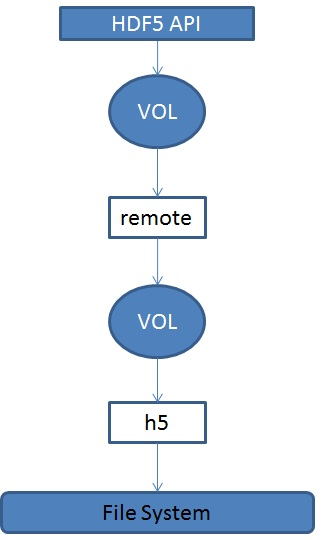
\includegraphics[width=90mm]{stacked.jpg}
\caption{Stacked VOL plugins.}
\label{stack}
\end{figure}

\subsection{Mirroring Plugins}
Another useful design option is to allow a mirroring plugin, where the
HDF5 API calls are forwarded through a mirror plugin to two or more
VOL plugins. This is an extention to the stacking
feature. Figure~\ref{mirror} shows an example of a VOL mirror that
maps HDF5 API calls to an h5 backend plugin and an XML backend plugin.

\begin{figure}[ht!]
\centering
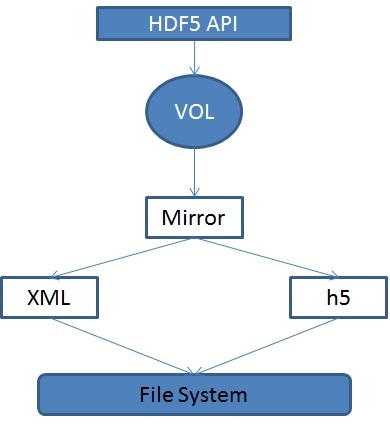
\includegraphics[width=90mm]{mirrored.jpg}
\caption{Mirrored VOL plugins.}
\label{mirror}
\end{figure}

Another possible VOL plugin could be a statistics plugin that just
gathers information on HDF5 API calls and records statistics
associated with the number of calls to a specific API functions and
corresponding parameters. This plugin would be very useful for
profiling purposes. The statistics plugin would be stacked on top of
another VOL plugin that actually performs the required access to the
file.

\subsection{Implementing Stacked and Mirrored Plugins}
A new set of API calls that map directly to the VOL callbacks have
been added to the HDF5 library to make stacking and mirroring easy for
plugin developers. Those APIs are listed at then end of Section~\ref{sec:api}. They are similar to the public VFD (H5FD) routines that call the VFD callbacks directly.

Using those new APIs, A mirror VOL plugin could, for example, implement the create callback in the file class by creating two HDF5 containers each with a different underlying plugin with 2 calls to:
\begin{lstlisting}
void *H5VLfile_create(const char *name, unsigned flags, hid_t fcpl_id, hid_t fapl_id, hid_t dxpl_id, void **req);
\end{lstlisting}
where each call uses a different file access property list, each with the VOL plugin property set to the underlying plugins. Then the mirror plugin creates a structure containing the pointers for the containers returned from both underlying plugins and returns a pointer to that structure as the output of the file create callback. Subsequent access to the container would again call the the public VOL routines twice for each plugin with its corresponding objects and combine the output as needed. 

%%% Local Variables: 
%%% mode: latex
%%% TeX-master: t
%%% End: 

\appendix
\section{VOL Plugin Example}
\label{sec:A}

This appendix shows a simple implementation of a {\tt printf} plugin that stacks on top of the native HDF5 plugin. Note that not all callbacks have been implemented since this is just an example for explaining the general framework of the VOL plugin.

\begin{lstlisting}

#include <stdio.h>
#include <stdlib.h>
#include <assert.h>
#include "hdf5.h"

#define LOG 502

static herr_t H5VL_log_init(hid_t vipl_id);
static herr_t H5VL_log_term(hid_t vtpl_id);

/* Datatype callbacks */
static void *H5VL_log_datatype_commit(void *obj, H5VL_loc_params_t loc_params, const char *name, hid_t type_id, hid_t lcpl_id, hid_t tcpl_id, hid_t tapl_id, hid_t dxpl_id, void **req);
static void *H5VL_log_datatype_open(void *obj, H5VL_loc_params_t loc_params, const char *name, hid_t tapl_id, hid_t dxpl_id, void **req);
static herr_t H5VL_log_datatype_get(void *dt, H5VL_datatype_get_t get_type, hid_t dxpl_id, void **req, va_list arguments);
static herr_t H5VL_log_datatype_close(void *dt, hid_t dxpl_id, void **req);

/* Dataset callbacks */
static void *H5VL_log_dataset_create(void *obj, H5VL_loc_params_t loc_params, const char *name, hid_t dcpl_id, hid_t dapl_id, hid_t dxpl_id, void **req);
static void *H5VL_log_dataset_open(void *obj, H5VL_loc_params_t loc_params, const char *name, hid_t dapl_id, hid_t dxpl_id, void **req);
static herr_t H5VL_log_dataset_read(void *dset, hid_t mem_type_id, hid_t mem_space_id,
                                    hid_t file_space_id, hid_t plist_id, void *buf, void **req);
static herr_t H5VL_log_dataset_write(void *dset, hid_t mem_type_id, hid_t mem_space_id,
                                     hid_t file_space_id, hid_t plist_id, const void *buf, void **req);
static herr_t H5VL_log_dataset_close(void *dset, hid_t dxpl_id, void **req);

/* File callbacks */
static void *H5VL_log_file_create(const char *name, unsigned flags, hid_t fcpl_id, hid_t fapl_id, hid_t dxpl_id, void **req);
static void *H5VL_log_file_open(const char *name, unsigned flags, hid_t fapl_id, hid_t dxpl_id, void **req);
static herr_t H5VL_log_file_get(void *file, H5VL_file_get_t get_type, hid_t dxpl_id, void **req, va_list arguments);
static herr_t H5VL_log_file_close(void *file, hid_t dxpl_id, void **req);

/* Group callbacks */
static void *H5VL_log_group_create(void *obj, H5VL_loc_params_t loc_params, const char *name, hid_t gcpl_id, hid_t gapl_id, hid_t dxpl_id, void **req);
static herr_t H5VL_log_group_close(void *grp, hid_t dxpl_id, void **req);

/* Link callbacks */

/* Object callbacks */
static void *H5VL_log_object_open(void *obj, H5VL_loc_params_t loc_params, H5I_type_t *opened_type, hid_t dxpl_id, void **req);
static herr_t H5VL_log_object_specific(void *obj, H5VL_loc_params_t loc_params, H5VL_object_specific_t specific_type, hid_t dxpl_id, void **req, va_list arguments);

hid_t native_plugin_id = -1;

static const H5VL_class_t H5VL_log_g = {
    0,
    LOG,
    "log",					/* name */
    H5VL_log_init,                              /* initialize */
    H5VL_log_term,                              /* terminate */
    sizeof(hid_t),
    NULL,
    NULL,
    {                                           /* attribute_cls */
        NULL, //H5VL_log_attr_create,                /* create */
        NULL, //H5VL_log_attr_open,                  /* open */
        NULL, //H5VL_log_attr_read,                  /* read */
        NULL, //H5VL_log_attr_write,                 /* write */
        NULL, //H5VL_log_attr_get,                   /* get */
        NULL, //H5VL_log_attr_specific,              /* specific */
        NULL, //H5VL_log_attr_optional,              /* optional */
        NULL  //H5VL_log_attr_close                  /* close */
    },
    {                                           /* dataset_cls */
        H5VL_log_dataset_create,                    /* create */
        H5VL_log_dataset_open,                      /* open */
        H5VL_log_dataset_read,                      /* read */
        H5VL_log_dataset_write,                     /* write */
        NULL, //H5VL_log_dataset_get,               /* get */
        NULL, //H5VL_log_dataset_specific,          /* specific */
        NULL, //H5VL_log_dataset_optional,          /* optional */
        H5VL_log_dataset_close                      /* close */
    },
    {                                               /* datatype_cls */
        H5VL_log_datatype_commit,                   /* commit */
        H5VL_log_datatype_open,                     /* open */
        H5VL_log_datatype_get,                      /* get_size */
        NULL, //H5VL_log_datatype_specific,         /* specific */
        NULL, //H5VL_log_datatype_optional,         /* optional */
        H5VL_log_datatype_close                     /* close */
    },
    {                                           /* file_cls */
        H5VL_log_file_create,                      /* create */
        H5VL_log_file_open,                        /* open */
        H5VL_log_file_get,                         /* get */
        NULL, //H5VL_log_file_specific,            /* specific */
        NULL, //H5VL_log_file_optional,            /* optional */
        H5VL_log_file_close                        /* close */
    },
    {                                           /* group_cls */
        H5VL_log_group_create,                     /* create */
        NULL, //H5VL_log_group_open,               /* open */
        NULL, //H5VL_log_group_get,                /* get */
        NULL, //H5VL_log_group_specific,           /* specific */
        NULL, //H5VL_log_group_optional,           /* optional */
        H5VL_log_group_close                       /* close */
    },
    {                                           /* link_cls */
        NULL, //H5VL_log_link_create,                /* create */
        NULL, //H5VL_log_link_copy,                  /* copy */
        NULL, //H5VL_log_link_move,                  /* move */
        NULL, //H5VL_log_link_get,                   /* get */
        NULL, //H5VL_log_link_specific,              /* specific */
        NULL, //H5VL_log_link_optional,              /* optional */
    },
    {                                           /* object_cls */
        H5VL_log_object_open,                        /* open */
        NULL, //H5VL_log_object_copy,                /* copy */
        NULL, //H5VL_log_object_get,                 /* get */
        H5VL_log_object_specific,                    /* specific */
        NULL, //H5VL_log_object_optional,            /* optional */
    },
    {
        NULL,
        NULL,
        NULL
    },
    NULL
};

typedef struct H5VL_log_t {
    void   *under_object;
} H5VL_log_t;

static herr_t
visit_cb(hid_t oid, const char *name,
         const H5O_info_t *oinfo, void *udata)
{
    ssize_t len;
    char n[25];

    if(H5Iget_type(oid) == H5I_GROUP) {
        len = H5VLget_plugin_name(oid, n, 50);
        printf ("Visiting GROUP VOL name = %s  %d\n", n, len);
    }
    if(H5Iget_type(oid) == H5I_DATASET) 
        printf("visiting dataset\n");
    if(H5Iget_type(oid) == H5I_DATATYPE) 
        printf("visiting datatype\n");

    return 1;
} /* end h5_verify_cached_stabs_cb() */

int main(int argc, char **argv) {
        const char file_name[]="large_dataset.h5";
	const char group_name[]="/Group";
	const char dataset_name[]="Data";
	char fullpath[500];
	hid_t file_id;
	hid_t group_id;
	hid_t dataspaceId;
        hid_t datasetId;
        hid_t acc_tpl;
        hid_t under_fapl;
        hid_t vol_id, vol_id2;
        hid_t int_id;
        hid_t attr;
        hid_t space;
	const unsigned int nelem=60;
	int *data;
	unsigned int i;
	hsize_t dims[1];
        ssize_t len;
        char name[25];
        static hsize_t      ds_size[2] = {10, 20};

        under_fapl = H5Pcreate (H5P_FILE_ACCESS);
        H5Pset_fapl_native(under_fapl);
        assert(H5VLis_registered("native") == 1);

        vol_id = H5VLregister (&H5VL_log_g);
        assert(vol_id > 0);
        assert(H5VLis_registered("log") == 1);

        vol_id2 = H5VLget_plugin_id("log");
        H5VLinitialize(vol_id2, H5P_DEFAULT);
        H5VLclose(vol_id2);

        native_plugin_id = H5VLget_plugin_id("native");
        assert(native_plugin_id > 0);

        acc_tpl = H5Pcreate (H5P_FILE_ACCESS);
        H5Pset_vol(acc_tpl, vol_id, &under_fapl);

	file_id = H5Fcreate(file_name, H5F_ACC_TRUNC, H5P_DEFAULT, acc_tpl);
        len = H5VLget_plugin_name(file_id, name, 25);
        printf ("FILE VOL name = %s  %d\n", name, len);

	group_id = H5Gcreate2(file_id, group_name, H5P_DEFAULT, H5P_DEFAULT, H5P_DEFAULT);
        len = H5VLget_plugin_name(group_id, name, 50);
        printf ("GROUP VOL name = %s  %d\n", name, len);

        int_id = H5Tcopy(H5T_NATIVE_INT);
        H5Tcommit2(file_id, "int", int_id, H5P_DEFAULT, H5P_DEFAULT, H5P_DEFAULT);
        len = H5VLget_plugin_name(int_id, name, 50);
        printf ("DT COMMIT name = %s  %d\n", name, len);
        H5Tclose(int_id);

        int_id = H5Topen2(file_id, "int", H5P_DEFAULT);
        len = H5VLget_plugin_name(int_id, name, 50);
        printf ("DT OPEN name = %s  %d\n", name, len);
        H5Tclose(int_id);

        int_id = H5Oopen(file_id,"int",H5P_DEFAULT);
        len = H5VLget_plugin_name(int_id, name, 50);
        printf ("DT OOPEN name = %s  %d\n", name, len);

        len = H5Fget_name(file_id, name, 50);
        printf("name = %d  %s\n", len, name);

	data = malloc (sizeof(int)*nelem);
	for(i=0;i<nelem;++i)
	  data[i]=i;

	dims [0] = 60;
	dataspaceId = H5Screate_simple(1, dims, NULL); 
        space = H5Screate_simple (2, ds_size, ds_size);

	sprintf(fullpath,"%s/%s",group_name,dataset_name);
	datasetId = H5Dcreate2(file_id, fullpath, H5T_NATIVE_INT, dataspaceId, H5P_DEFAULT, H5P_DEFAULT, H5P_DEFAULT);
	H5Sclose(dataspaceId);

        len = H5VLget_plugin_name(datasetId, name, 50);
        printf ("DSET name = %s  %d\n", name, len);

	H5Dwrite(datasetId, H5T_NATIVE_INT, H5S_ALL, H5S_ALL, H5P_DEFAULT, data);
	H5Dclose(datasetId);

        H5Ovisit(file_id, H5_INDEX_NAME, H5_ITER_NATIVE, visit_cb, NULL);

	free (data);
        H5Oclose(int_id);
        H5Sclose (space);
	H5Gclose(group_id);

	H5Fclose(file_id);
        H5Pclose(acc_tpl);
        H5Pclose(under_fapl);

        H5VLclose(native_plugin_id);
        H5VLterminate(vol_id, H5P_DEFAULT);
        H5VLunregister (vol_id);
        assert(H5VLis_registered("log") == 0);
	return 0;
}

static herr_t H5VL_log_init(hid_t vipl_id)
{
    printf("------- LOG INIT\n");
    return 0;
}

static herr_t H5VL_log_term(hid_t vtpl_id)
{
    printf("------- LOG TERM\n");
    return 0;
}

static void *
H5VL_log_file_create(const char *name, unsigned flags, hid_t fcpl_id, hid_t fapl_id, hid_t dxpl_id, void **req)
{
    hid_t under_fapl;
    H5VL_log_t *file;

    file = (H5VL_log_t *)calloc(1, sizeof(H5VL_log_t));

    under_fapl = *((hid_t *)H5Pget_vol_info(fapl_id));
    file->under_object = H5VLfile_create(name, flags, fcpl_id, under_fapl, dxpl_id, req);

    printf("------- LOG H5Fcreate\n");
    return (void *)file;
}

static void *
H5VL_log_file_open(const char *name, unsigned flags, hid_t fapl_id, hid_t dxpl_id, void **req)
{
    hid_t under_fapl;
    H5VL_log_t *file;

    file = (H5VL_log_t *)calloc(1, sizeof(H5VL_log_t));

    under_fapl = *((hid_t *)H5Pget_vol_info(fapl_id));
    file->under_object = H5VLfile_open(name, flags, under_fapl, dxpl_id, req);

    printf("------- LOG H5Fopen\n");
    return (void *)file;
}

static herr_t 
H5VL_log_file_get(void *file, H5VL_file_get_t get_type, hid_t dxpl_id, void **req, va_list arguments)
{
    H5VL_log_t *f = (H5VL_log_t *)file;

    H5VLfile_get(f->under_object, native_plugin_id, get_type, dxpl_id, req, arguments);

    printf("------- LOG H5Fget %d\n", get_type);
    return 1;
}
static herr_t 
H5VL_log_file_close(void *file, hid_t dxpl_id, void **req)
{
    H5VL_log_t *f = (H5VL_log_t *)file;

    H5VLfile_close(f->under_object, native_plugin_id, dxpl_id, req);
    free(f);

    printf("------- LOG H5Fclose\n");
    return 1;
}

static void *
H5VL_log_group_create(void *obj, H5VL_loc_params_t loc_params, const char *name, 
                      hid_t gcpl_id, hid_t gapl_id, hid_t dxpl_id, void **req)
{
    H5VL_log_t *group;
    H5VL_log_t *o = (H5VL_log_t *)obj;

    group = (H5VL_log_t *)calloc(1, sizeof(H5VL_log_t));

    group->under_object = H5VLgroup_create(o->under_object, loc_params, native_plugin_id, name, gcpl_id,  gapl_id, dxpl_id, req);

    printf("------- LOG H5Gcreate\n");
    return (void *)group;
}

static herr_t 
H5VL_log_group_close(void *grp, hid_t dxpl_id, void **req)
{
    H5VL_log_t *g = (H5VL_log_t *)grp;

    H5VLgroup_close(g->under_object, native_plugin_id, dxpl_id, req);
    free(g);

    printf("------- LOG H5Gclose\n");
    return 1;
}

static void *
H5VL_log_datatype_commit(void *obj, H5VL_loc_params_t loc_params, const char *name, 
                         hid_t type_id, hid_t lcpl_id, hid_t tcpl_id, hid_t tapl_id, hid_t dxpl_id, void **req)
{
    H5VL_log_t *dt;
    H5VL_log_t *o = (H5VL_log_t *)obj;

    dt = (H5VL_log_t *)calloc(1, sizeof(H5VL_log_t));

    dt->under_object = H5VLdatatype_commit(o->under_object, loc_params, native_plugin_id, name, 
                                           type_id, lcpl_id, tcpl_id, tapl_id, dxpl_id, req);

    printf("------- LOG H5Tcommit\n");
    return dt;
}
static void *
H5VL_log_datatype_open(void *obj, H5VL_loc_params_t loc_params, const char *name, hid_t tapl_id, hid_t dxpl_id, void **req)
{
    H5VL_log_t *dt;
    H5VL_log_t *o = (H5VL_log_t *)obj;  

    dt = (H5VL_log_t *)calloc(1, sizeof(H5VL_log_t));

    dt->under_object = H5VLdatatype_open(o->under_object, loc_params, native_plugin_id, name, tapl_id, dxpl_id, req);

    printf("------- LOG H5Topen\n");
    return (void *)dt;
}

static herr_t 
H5VL_log_datatype_get(void *dt, H5VL_datatype_get_t get_type, hid_t dxpl_id, void **req, va_list arguments)
{
    H5VL_log_t *o = (H5VL_log_t *)dt;
    herr_t ret_value;

    ret_value = H5VLdatatype_get(o->under_object, native_plugin_id, get_type, dxpl_id, req, arguments);

    printf("------- LOG datatype get\n");
    return ret_value;
}

static herr_t 
H5VL_log_datatype_close(void *dt, hid_t dxpl_id, void **req)
{
    H5VL_log_t *type = (H5VL_log_t *)dt;

    assert(type->under_object);

    H5VLdatatype_close(type->under_object, native_plugin_id, dxpl_id, req);
    free(type);

    printf("------- LOG H5Tclose\n");
    return 1;
}

static void *
H5VL_log_object_open(void *obj, H5VL_loc_params_t loc_params, H5I_type_t *opened_type, hid_t dxpl_id, void **req)
{
    H5VL_log_t *new_obj;
    H5VL_log_t *o = (H5VL_log_t *)obj;

    new_obj = (H5VL_log_t *)calloc(1, sizeof(H5VL_log_t));
    
    new_obj->under_object = H5VLobject_open(o->under_object, loc_params, native_plugin_id, opened_type, dxpl_id, req);

    printf("------- LOG H5Oopen\n");
    return (void *)new_obj;
}

static herr_t 
H5VL_log_object_specific(void *obj, H5VL_loc_params_t loc_params, H5VL_object_specific_t specific_type, 
                         hid_t dxpl_id, void **req, va_list arguments)
{
    H5VL_log_t *o = (H5VL_log_t *)obj;

    H5VLobject_specific(o->under_object, loc_params, native_plugin_id, specific_type, dxpl_id, req, arguments);

    printf("------- LOG Object specific\n");
    return 1;
}

static void *
H5VL_log_dataset_create(void *obj, H5VL_loc_params_t loc_params, const char *name, hid_t dcpl_id, hid_t dapl_id, hid_t dxpl_id, void **req) 
{
    H5VL_log_t *dset;
    H5VL_log_t *o = (H5VL_log_t *)obj;

    dset = (H5VL_log_t *)calloc(1, sizeof(H5VL_log_t));

    dset->under_object = H5VLdataset_create(o->under_object, loc_params, native_plugin_id, name, dcpl_id,  dapl_id, dxpl_id, req);

    printf("------- LOG H5Dcreate\n");
    return (void *)dset;
}

static void *
H5VL_log_dataset_open(void *obj, H5VL_loc_params_t loc_params, const char *name, hid_t dapl_id, hid_t dxpl_id, void **req)
{
    H5VL_log_t *dset;
    H5VL_log_t *o = (H5VL_log_t *)obj;

    dset = (H5VL_log_t *)calloc(1, sizeof(H5VL_log_t));

    dset->under_object = H5VLdataset_open(o->under_object, loc_params, native_plugin_id, name, dapl_id, dxpl_id, req);

    printf("------- LOG H5Dopen\n");
    return (void *)dset;
}

static herr_t 
H5VL_log_dataset_read(void *dset, hid_t mem_type_id, hid_t mem_space_id,
                      hid_t file_space_id, hid_t plist_id, void *buf, void **req)
{
    H5VL_log_t *d = (H5VL_log_t *)dset;

    H5VLdataset_read(d->under_object, native_plugin_id, mem_type_id, mem_space_id, file_space_id, 
                     plist_id, buf, req);

    printf("------- LOG H5Dread\n");
    return 1;
}
static herr_t 
H5VL_log_dataset_write(void *dset, hid_t mem_type_id, hid_t mem_space_id,
                       hid_t file_space_id, hid_t plist_id, const void *buf, void **req)
{
    H5VL_log_t *d = (H5VL_log_t *)dset;

    H5VLdataset_write(d->under_object, native_plugin_id, mem_type_id, mem_space_id, file_space_id, 
                     plist_id, buf, req);

    printf("------- LOG H5Dwrite\n");
    return 1;
}
static herr_t 
H5VL_log_dataset_close(void *dset, hid_t dxpl_id, void **req)
{
    H5VL_log_t *d = (H5VL_log_t *)dset;

    H5VLdataset_close(d->under_object, native_plugin_id, dxpl_id, req);
    free(d);

    printf("------- LOG H5Dclose\n");
    return 1;
}
\end{lstlisting}

%%% Local Variables: 
%%% mode: latex
%%% TeX-master: t
%%% End: 


%% References
\bibliography{IEEEabrv,main}
\bibliographystyle{IEEEtran}

\end{document}
